\documentclass[lettersize,journal]{IEEEtran}
\usepackage{amsmath,amsfonts}
\usepackage{algorithmic}
\usepackage{algorithm}
\usepackage{array}
\usepackage[caption=false,font=normalsize,labelfont=sf,textfont=sf]{subfig}
\usepackage{textcomp}
\usepackage{stfloats}
\usepackage{url}
\usepackage{verbatim}
\usepackage{graphicx}
\usepackage{cite}

% Our additions - Laplacian Analysis
\usepackage{hyperref}
\usepackage{multirow}
\usepackage{booktabs}

\hyphenation{op-tical net-works semi-conduc-tor IEEE-Xplore}
% updated with editorial comments 8/9/2021

\begin{document}
\title{Analysis of Laplacian Interpolation and Deformation Vector Field Optimization Towards Invertible Image Registration}

\author{
        {Andy Thai, University of California, Irvine},

        {Gnana Heemmanshuu Dasari, University of California, Irvine},

        {Xiangmin Xu, University of California, Irvine},
        
        {M. Gopi, University of California, Irvine}
}

% The paper headers
\markboth{Journal of \LaTeX\ Class Files,~Vol.~14, No.~8, August~2021}%
{Shell \MakeLowercase{\textit{et al.}}: A Sample Article Using IEEEtran.cls for IEEE Journals}

\IEEEpubid{0000--0000/00\$00.00~\copyright~2021 IEEE}
% Remember, if you use this you must call \IEEEpubidadjcol in the second
% column for its text to clear the IEEEpubid mark.

\maketitle

\begin{abstract}
Accurate and invertible image registration remains a core challenge in biomedical imaging applications. Laplacian interpolation is popular for its ability to estimate dense deformation fields from sparse point correspondences, which can be used to deform a microscopic image, called the moving image, towards a target or template image, also called the fixed image. These deformations can be done either space, mapping from moving to fixed, or fixed to moving, with pros and cons between each direction of mapping. However, these deformations are prone to non-invertible transformations, especially in regions with conflicting or undersampled correspondences. Non-invertible transformations may be due to many reasons, including numerical errors, incorrect or outliers in correspondences, as well as inflexibility in the interpolation function to detect and avoid non-invertible mappings. Our goal in this paper is to analyze and address non-invertibility that stems primarily from numerical errors and, in that context, change the interpolation function to reduce many-to-one non-invertible mappings.

We first analyze the role of interpolation space (fixed versus moving) and note potential issues such as smearing and duplication artifacts that may arise in using interpolation in fixed space.
We then propose a method for modifying the deformation field by using displacement information computed using Laplacian interpolation between the moving and fixed image domains in specific regions. Specifically, we identify areas of local expansion in one image using the Jacobian determinant, and use point-to-point mappings in those areas to create new augmented correspondences. These augmented correspondences can be combined with the initial set of correspondences to compute a new deformation field result with reduced non-invertible mappings.

We evaluate our approach on synthetic and real mouse brain image data, showing that it can significantly reduce the number of non-positive Jacobian determinants and improve the invertibility of the resulting transformation.  Our findings suggest that utilizing both interpolation space and the augmentation of correspondence sets can be critical in ensuring diffeomorphic and correct image registration.

\end{abstract}


%\keywords{Laplacian, registration, Jacobian determinant, deformation, invertibility, correspondence, interpolation}
\begin{IEEEkeywords}
Laplacian, registration, Jacobian determinant, deformation, invertibility, correspondence, interpolation.
\end{IEEEkeywords}







\section{Introduction}

Image registration is a critical process in biomedical imaging, where spatial correspondences are established between a moving and a fixed image to align anatomical or functional structures. A key step in many registration approaches is the interpolation of sparse landmark correspondences to form a dense and smooth deformation field, which can be performed with Laplacian interpolation. This interpolation can be computed in either of the two image domains: $M\rightarrow F$, if the interpolation is done in the moving space, or $F\rightarrow M$ if it is done in the fixed space.

This interpolation behavior depends heavily on the choice of coordinate space. When interpolation is performed in the fixed image space ($F\rightarrow M$), artifacts such as blurring, smearing, and duplication of features can arise. These are caused by the fact that displacements are interpolated across the domain, and not correspondences, which may lead to many-to-one mappings from the fixed image to the moving image. The moving image being used as a "texture map" with many-to-one mappings from the fixed image would result in duplication of moving image content or hollowed-out regions in the output.

In contrast, performing Laplacian interpolation in the moving image space ensures an injective relationship between the moving image and the output and can avoid these artifacts. Because the interpolation and subsequent deformation operations take place in the image being deformed, expansion and compression are naturally encoded by the deformation itself.

However, regardless of domain choice in interpolation, a common challenge in registration is ensuring that the resulting mapping is both smooth and invertible, meaning it must preserve topology and avoid non-physical distortions, such as folding. During registration between two image spaces, say, a moving and fixed image, a few sparse correspondences between these images are given, and the rest of the correspondences for the entire space are computed using an interpolatory mapping function. We use Laplacian interpolation to interpolate deformation vectors (not correspondences directly), adding a deformation vector to a point in one image to obtain its corresponding point in the other image. Such correspondence mappings may or may not be invertible. Our focus is to make this correspondence mapping as invertible as possible. 

\begin{figure*}[ht]
    \centering
    
\includegraphics[width=0.24\linewidth]{images/laplacian_analysis/registration/microscopic_section.png}
    
\includegraphics[width=0.24\linewidth]{images/laplacian_analysis/registration/template_section.png}
    
\includegraphics[width=0.24\linewidth]{images/laplacian_analysis/registration/pre_reg.png}
    
\includegraphics[width=0.24\linewidth]{images/laplacian_analysis/registration/post_reg.png}
    \caption{An example of a registration operation is depicted. The first image shows a microscopic image, which is to be aligned and deformed to an Allen CCF averaged template section in the second image. The third image depicts the microscopic image with the template section boundary labels overlaid. The fourth image depicts the result of registration to the template section with the boundary labels overlaid.}
    \label{fig:registration-example}
\end{figure*}

An important property we can use is to accomplish this goal is {\it symmetry}. As mentioned above, the interpolation of correspondences (or the deformation vectors) can be done either in the moving image space ($M\rightarrow F$) or the fixed image space ($F\rightarrow M$). When both mappings are computed independently, the resulting correspondences after interpolation may not be symmetric: that is, the mappings $M\rightarrow F$ and $F\rightarrow M$ may not be inverses of each other. (This is different from each of these two mappings being independently invertible.) This property provides new information can be leveraged to target regions of interest to further promote local invertibility in deformation vector fields and reduce numerical error.

To address these main points of interpolatory spaces and invertibility in our work, we showcase differences in real-world examples where Laplacian interpolation is applied in both fixed and moving image domains and compare the outputs to popular registration toolkits such as ANTs \cite{AVANTS200826} and Elastix \cite{Klein2010elastixAT} that perform deformation in the fixed image space. We then propose a method to force local symmetry in specific regions to reduce numerical errors in correspondence (or deformation vector) interpolation and thus to improve invertibility.

\subsection{Main contributions}
\label{subsec:main_contributions}

Our main contributions can be summarized as follows:

\textbf{Analysis of non-invertibility and interpolatory spaces}: We define folding artifacts and analyze factors that can lead to folding in registration and in subsequent deformation vector fields. Additionally, we explore the difference between performing Laplacian interpolation in the moving and the fixed image spaces, and review the drawbacks of interpolating over fixed image domains.

\textbf{Improving invertibility of registration mapping}: We present a method to update and augment correspondences in Laplacian interpolated deformation vector fields. By sharing, in specific chosen regions, more contextual information from interpolated deformation fields in the moving and fixed image spaces, we can incorporate the correspondence mappings such that more local Jacobian determinants are positive. This operation preserves the visual fidelity of the registered image, as it includes only additional interpolated correspondences, and changes minimally from the initial computed Laplacian deformation vector field.


\section{Related work}
\label{sec:related_work}

\autoref{fig:registration-example} shows a microscopic image (moving image), a template image (fixed image), and their registration. Warping or deforming the moving image to register with the fixed image such that anatomical and functional regions of the moving image align with the fixed image is the goal of all image registration techniques. Registration methods and invertibility of deformations \cite{Dupuis1998}, especially in biomedical imaging literature, have a long history, and many review papers offer an in-depth overview of these developments \cite{KLEIN2009786}.

\textbf{Rigid registration.}
Rigid registration in image alignment is comprised of only translation and rotation operations without any scaling or deformation in 2D or 3D space \cite{Zhang1994IterativePM}. Its use cases assume that the anatomical structures of interest remain unchanged in shape and size across images, making it suitable for scenarios such as longitudinal studies of the same subject \cite{REUTER20101181}. These invertible transforms may also be used in preprocessing as coarse alignments for subsequent non-rigid transformations \cite{Frackowiak2004-yy}.

\textbf{Non-rigid registration.}
Within these non-rigid transformations, pixel/voxel-wise intensity comparisons are typically utilized. By maximizing energy functionals or similarity measures on these intensity values, they can avoid requiring feature extraction or correspondence detection \cite{regreviewsong}. To ensure smooth and plausible deformations, these energy functionals are commonly regularized, which helps prevent folding and unrealistic warping \cite{Reithmeir2024}. This approach makes intensity-based registration broadly applicable, being able to handle free-form registration problems with B-splines \cite{Rueckert1999} or stochastic methods \cite{Tustison2009}.

Landmark-based registration methods \cite{MAINTZ19981, ZITOVA2003977} establish some form of correspondence mapping, which can span from points/voxel pairs or to subregional patches \cite{Ourselin2000BlockMA,PatchBasedRegistration} on edges and boundaries between image domains. Registration and spatial transformations around these correspondences can achieve accurate and fine alignment with the use of interpolation techniques \cite{ALLASIA20141}, such as thin-plate splines \cite{Sun2011} or Laplacian operators \cite{AgarwalRobustRegistration, AgarwalXG16, AGARWAL201845, RegBoost2025}. However, this leads to the drawback of these landmark-based mappings potentially not guaranteeing diffeomorphic outputs, motivating diffeomorphic methods such as \cite{Beg2005,THIRION1998243,VERCAUTEREN2009S61,sphericaldemons}. In some of these works, correspondences may be regularized \cite{Shusharina2012-ez} or used alongside variational and diffeomorphic algorithms as \cite{ASHBURNER200795, AVANTS200826, VERCAUTEREN2009S61}, often seen in toolboxes such as ANTs \cite{AVANTS200826} and Elastix \cite{Klein2010elastixAT}. 


%Landmark-based registration methods \cite{MAINTZ19981, ZITOVA2003977} establish discrete correspondences between points, patches \cite{PatchBasedRegistration}, or regions \cite{Ourselin2000BlockMA} in a moving image and a fixed template domain. These correspondences typically capture key anatomical structures, such as shape boundaries or regions of interest. Precise local alignment is achieved near these landmarks, while transformations in the surrounding areas are often estimated using interpolation techniques \cite{ALLASIA20141}, including thin-plate splines \cite{Sun2011} and Laplacian operators \cite{AgarwalRobustRegistration, AgarwalXG16, AGARWAL201845, RegBoost2025}.


\textbf{Laplacian.}
Laplacian formulations in particular, have been successfully used and applied to biomedical image datasets like mouse brain data. The works of \cite{AgarwalRobustRegistration, AgarwalXG16, AGARWAL201845} establish correspondences between sectioned mouse brain images and the Allen Mouse Brain Common Coordinate Framework template \cite{WANG2020936}, utilizing a Laplacian formulation to solve for displacements. \cite{RegBoost2025} extends this work to 3D volumes, providing smooth transitions between brain sections and offering improvements upon existing registration frameworks.


%However, these methods may have high runtimes due to numerical integration and high-dimensional parameter spaces, making them unsuitable for large datasets. Additionally, these methods can be sensitive to noise, and significant variation between registration pairs can introduce difficulties, as similarity measures are typically non-convex and may get trapped in local minima, relying on initialization methods such as pose estimation \cite{VARNAVAS2015108} or shape-encoding \cite{Miao2013}. Thus, these methods are not as easily scalable to very large-scale pipelines.

\textbf{Learning-based methods.}
Recent trends have shifted towards learning-based image registration frameworks to estimate deformation fields. Works such as VoxelMorph \cite{VoxelMorph2019} leverage convolutional neural networks and similarity-based smoothness loss functions to achieve extremely fast computations with GPU hardware, with many other works building off of the model \cite{Hoopes2021HyperMorph, hoffmann2022synthmorph, CHEN2022102615}.

However, although learning-based frameworks can output fast results, they do not inherently guarantee diffeomorphic outputs, and the resultant deformation fields may contain folding artifacts. Recent developments in learning-based models currently focus on minimizing these occurrences through regularization and architectural design \cite{Dalca2018, KIM2021CycleMorph, Huang2023} to encourage bidirectional consistency, but cannot guarantee complete invertibility. Ensuring this property remains an active problem for deep learning-based approaches.



\begin{comment}
As a result, much work exists that aims to reduce the amount of local folding within registration operations (represented by non-positive Jacobian determinant values), ranging from the methods previously discussed in diffeomorphic models to cycle-consistency, each with its unique benefits and drawbacks. However, many of these works that regularize invertibility, often seen in deep learning or when working with data where some regions are highly non-linear, can significantly reduce the amount of non-positive Jacobian determinants within DVFs to even near-zero and increase stability, but do not guarantee the output is completely free of non positive Jacobian determinant values. There has been some work in processing with matrix exponentials \cite{Pal2022} and architectural modules \cite{kuang2019reducingnegativejacobiandeterminant}, but research in processing DVFs post hoc is sparse. 
\end{comment}

\textbf{Our method.} 
Our work reduces the number of points with non-invertible mappings that are introduced due to possible numerical errors, while preserving visual fidelity in the registration. We demonstrate our method on deformations achieved using Laplacian interpolation, a popular landmark-based interpolation approach.    
Our method builds off of the work of \cite{AgarwalRobustRegistration, RegBoost2025} and enhances the invertibility of the deformation field outputs by utilizing additional information garnered from creating augmented correspondences based solely on the information from the original set of correspondences, minimizing the deviation from the initial correspondences.


% METHODS SECTION
\section{Laplacian and Jacobian}

% SECTION TO EXPLAIN REGISTRATION AND LAPLACIAN SETUP
\subsection{Registration with Laplacian function-based deformation fields}
\label{sec:laplacian_registration}

We define image registration as warping a moving image to a fixed image \cite{Yushkevich2023}. Let $\Omega$ and $\Omega'$ denote the set of coordinates of the moving image and fixed image, respectively. The image registration function $r$ is given by 
\begin{equation} \label{eq:image_registration_definition}
    r: \Omega \rightarrow \Omega'.
\end{equation}

The deformation vector field $\phi$, defined over the set $\Omega$, is defined as 
\begin{equation} \label{eq:dvf_definition}
    \text{for all } p \in \Omega, \quad \phi(p)=r(p)-p.
\end{equation}

Laplacian function-based registration \cite{RegBoost2025} computes a deformation field $\phi$ that transforms the space $\Omega$ to $\Omega'$ by interpolating a given sparse set of deformation vectors to the entire $\Omega$. This vector field consists of displacement vectors for each pixel in $\Omega$, which, when applied, transforms the pixel to its corresponding pixel in $\Omega'$. 

The Laplacian interpolation is done by solving Laplace's equation in \autoref{eq:laplace_eq1}:

\begin{equation} \label{eq:laplace_eq1}
\nabla^2 \phi = 0.
\end{equation}

Intuitively, the Laplacian linearly interpolates the deformation vector $\phi$, so that its second derivative is zero. We consider the displacements in each axis independent of the other and derive the following definitions in \autoref{eq:laplace_eq2}. 

\begin{equation} \label{eq:laplace_eq2}
\nabla^2 \phi_x = 0, \quad \nabla^2 \phi_y = 0.
\end{equation}

On images, we approximate the discrete Laplacian operator $\nabla^2$ using the finite difference method in 2D, which is given by 
\begin{equation} 
%\begin{align}
    \begin{split} \label{eq:laplacian_2d}
    \nabla^2 \phi \quad = \quad & \frac{1}{2}\phi(x + 1, y)+ \frac{1}{2} \phi(x - 1, y)\quad+\\ 
    & \frac{1}{2}\phi(x, y + 1) + \frac{1}{2}\phi(x, y - 1) - 2\cdot\phi(x, y) \quad \\
    = 0.
    \end{split} 
%\end{align}
\end{equation}

The above equation holds for every point (pixel) in the 2D space (image), which, when put together, can be expressed as a system of linear equations $A\phi=0$, where displacement values $\phi$ ($\phi_x$ or $\phi_y$) for each pixel are the unknown vector. The row vectors of $A$ are the coefficients of the $\phi$ values in \autoref{eq:laplacian_2d}. 

Additionally, we have constraints from the given correspondences. Let $C_m = (u, v)$ represent the set of points in $\Omega$ that have correspondences to $C_f = (u', v')$ in $\Omega'$. This gives the Dirichlet boundary conditions, as depicted in \autoref{eq:dirichlet_boundary_moving}.

\begin{align} \label{eq:dirichlet_boundary_moving}
    \begin{split}
    \phi(C_m)  =  (d_x, d_y) \quad = \quad & C_f - C_m \\
    B_x \quad = \quad &  u' - u, \\
    B_y \quad = \quad &  v' - v. \\
    \end{split}
\end{align}

Alternatively, when computing for the backward mapping (from the fixed space $\Omega'$ to the moving space $\Omega$), the Dirichlet boundary conditions can be represented as

\begin{align} \label{eq:dirichlet_boundary_fixed}
    \begin{split}
    \phi(C_f)  =  (d_x, d_y) \quad = \quad & C_m - C_f \\
    B_x \quad = \quad &  u - u', \\
    B_y \quad = \quad &  v - v'. \\
    \end{split}
\end{align}

Combining the above equations in \autoref{eq:dirichlet_boundary_moving} (or \autoref{eq:dirichlet_boundary_fixed}) with \autoref{eq:laplacian_2d}, we can form a linear system of equations in \autoref{eq:dirichlet_linear_system}.
\begin{align} \label{eq:dirichlet_linear_system}
    \begin{split}
    A\phi_x - B_x \quad = \quad & 0, \\
    A\phi_y - B_y \quad = \quad & 0.
    \end{split}
\end{align}   


The row vectors of A take the coefficients of terms in \autoref{eq:laplacian_2d}, except for the rows corresponding to points in $C_m$, in which case, they represent the Dirichlet boundary condition. The vectors $B_x$ and $B_y$ are zero everywhere except for the rows corresponding to $C_m$, in which case it is $d_x$ and $d_y$, respectively. 


% SECTION TO EXPLAIN JACOBIAN DETERMINANTS
\subsection{Invertibility and Jacobian determinants}
\label{sec:jacobian_determinants}

The Jacobian matrix of a vector-valued function such as $r$ in \autoref{eq:image_registration_definition} is a matrix representing the gradients of each component of a function in each direction. 
Let $\Omega, \Omega' \subset \mathbb{R}^n$ and $r$ is an $n$ dimensional mapping. The Jacobian matrix $J$ of the registration function $r$ is given by

% Generalized Jacobian formula for some function f
\begin{equation} \label{eq:general_jacobian_matrix}
    J = 
    \left( 
        \begin{bmatrix}
            \frac{\partial r_1}{\partial x_1} & \cdots & \frac{\partial r_1}{\partial x_n} \\
            \frac{\partial r_2}{\partial x_1} & \cdots & \frac{\partial r_2}{\partial x_n} \\
            \vdots & \ddots & \vdots \\
            \frac{\partial r_n}{\partial x_1} & \cdots & \frac{\partial r_n}{\partial x_n}
        \end{bmatrix}
    \right).
\end{equation}

A key focus of our analysis is the issue of invertibility of the registration mapping $r$. Interestingly, the determinant of the Jacobian of the mapping $r$ measures change in area. The Jacobian determinant value being greater than 1.0 represents area expansion, while values between 0 and 1.0 represent area contraction. Jacobian determinant values that are less than 0 indicate local folding and violate the one-to-one mapping assumption critical for many tasks, including longitudinal analysis and feature tracking. At these points with negative Jacobian determinants, the mapping $r$ becomes non-invertible.

 %From \autoref{eq:dvf_definition}, we denote $\det(J)$ to be the Jacobian determinant caused by the deformation $v$. The Jacobian determinant measures the local expansion or compression around a pixel $p$. A value greater than 1 implies expansion, between 0 and 1 implies compression, equal to 0 indicates collapse, and $<0$ indicates folding. Thus, an invertible transformation would have a positive value for the Jacobian determinant at all points in the domain. The generalized formulation of the determinant of the Jacobian matrix at point $(x_1, x_2, \ldots, x_n)$ is given by 

% Generalized Jacobian formula for some function f
\begin{equation} \label{eq:general_jacobian_matrix_det}
    \det(J_r) = 
    \det\left( 
        \begin{bmatrix}
            \frac{\partial r_1}{\partial x_1} & \cdots & \frac{\partial r_1}{\partial x_n} \\
            \frac{\partial r_2}{\partial x_1} & \cdots & \frac{\partial r_2}{\partial x_n} \\
            \vdots & \ddots & \vdots \\
            \frac{\partial r_n}{\partial x_1} & \cdots & \frac{\partial r_n}{\partial x_n}
        \end{bmatrix}
    \right).
\end{equation}

Rewriting the determinant of the Jacobian (\autoref{eq:general_jacobian_matrix_det}) for use with 2D digital images and replacing $r(p)$ with $\phi(p)+p$ using \autoref{eq:dvf_definition} gives \autoref{eq:2d_jacobian_matrix_det} for the determinant of a 2D discrete Jacobian matrix.

\begin{equation} \label{eq:2d_jacobian_matrix_det}
    \det(J_{r}) = 
    \det\left( 
    \begin{bmatrix}
    \frac{\partial \phi_x}{\partial x} + 1 & \frac{\partial \phi_x}{\partial y} \\
    \frac{\partial \phi_y}{\partial x} & \frac{\partial \phi_y}{\partial y} + 1
    \end{bmatrix}
    \right).
\end{equation}

The entries in the Jacobian matrix $J_{\phi}$ can be approximated for any given discretized point $(x, y)$ in a grid using the central differences method as in \autoref{eq:central_differences}, or the finite difference formula as in \autoref{eq:finite_differences} for the image boundary cases.

\begin{equation} \label{eq:central_differences}
    \begin{aligned}
        & \frac{\partial \phi_x}{\partial x} = \frac{\phi_x(x + 1, y) - \phi_x(x - 1, y)}{2} \\
        & \frac{\partial \phi_x}{\partial y} = \frac{\phi_x(x, y + 1) - \phi_x(x, y - 1)}{2} \\
        & \frac{\partial \phi_y}{\partial x} = \frac{\phi_y(x + 1, y) - \phi_y(x - 1, y)}{2} \\
        & \frac{\partial \phi_y}{\partial y} = \frac{\phi_y(x, y + 1) - \phi_y(x, y - 1)}{2}. \\
    \end{aligned}
\end{equation}

\begin{equation} \label{eq:finite_differences}
    \begin{aligned}
        & \frac{\partial \phi_x}{\partial x} = \phi_x(x + 1, y) - \phi_x(x, y), \hspace{0.05in}
        & \frac{\partial \phi_x}{\partial y} = \phi_x(x, y + 1) - \phi_x(x, y), \\
        & \frac{\partial \phi_y}{\partial x} = \phi_y(x + 1, y) - \phi_y(x, y), \hspace{0.05in}
        & \frac{\partial \phi_y}{\partial y} = \phi_y(x, y + 1) - \phi_y(x, y). \\
    \end{aligned}
\end{equation}

%With most computed deformation vector fields, the Jacobian determinant is not positive at all points on the grid. It is at these points that folding occurs, rendering the deformation field non-invertible and thus not diffeomorphic, as seen in \autoref{fig:correspondences}. 

%In addition to the number of non-positive Jacobian determinants present in a deformation vector field, the minimum Jacobian determinant value $\min (\det{(J_v)})$ in non-invertible deformation fields provides a measure of the severity of folding artifacts for the worst-case neighborhood.

\begin{figure*}[ht]
    \centering
    \setlength{\tabcolsep}{2pt}
    \renewcommand{\arraystretch}{1.8} % a bit more headroom

    \begin{tabular}{|c c|c|c|c|c|}
        \hline
        % ===== Header row 1 =====
        \multicolumn{2}{|c|}{\textbf{Input images}} &
        \multirow{2}{*}{\shortstack{\textbf{Results of}\\\textbf{interpolating in}\\\textbf{fixed image space}}} &
        \multirow{2}{*}{\shortstack{\textbf{Results of}\\\textbf{interpolating in}\\\textbf{moving image space}}} &
        \multirow{2}{*}{\shortstack{\textbf{Results of}\\\textbf{interpolating in}\\\textbf{ANTs SyN}}} &
        \multirow{2}{*}{\shortstack{\textbf{Results of}\\\textbf{interpolating in}\\\textbf{Elastix}}} \\
        % ===== Header row 2 (no \cline) =====
        \shortstack{\textbf{Moving}\\\textbf{image}} &
        \shortstack{\textbf{Fixed}\\\textbf{image}} &
        & & & \\[-0.3em] % trim vertical space before images
        \hline

        % ===== First row of images =====
        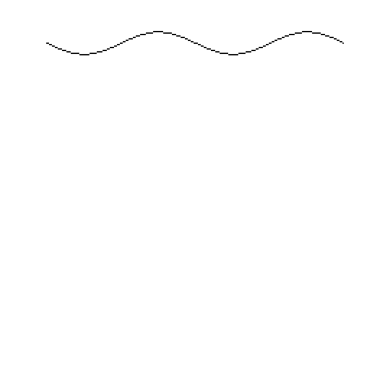
\includegraphics[width=0.155\linewidth]{images/laplacian_analysis/ants/moving_image_separate.png} &
        
\includegraphics[width=0.155\linewidth]{images/laplacian_analysis/ants/fixed_image_separate.png} &
        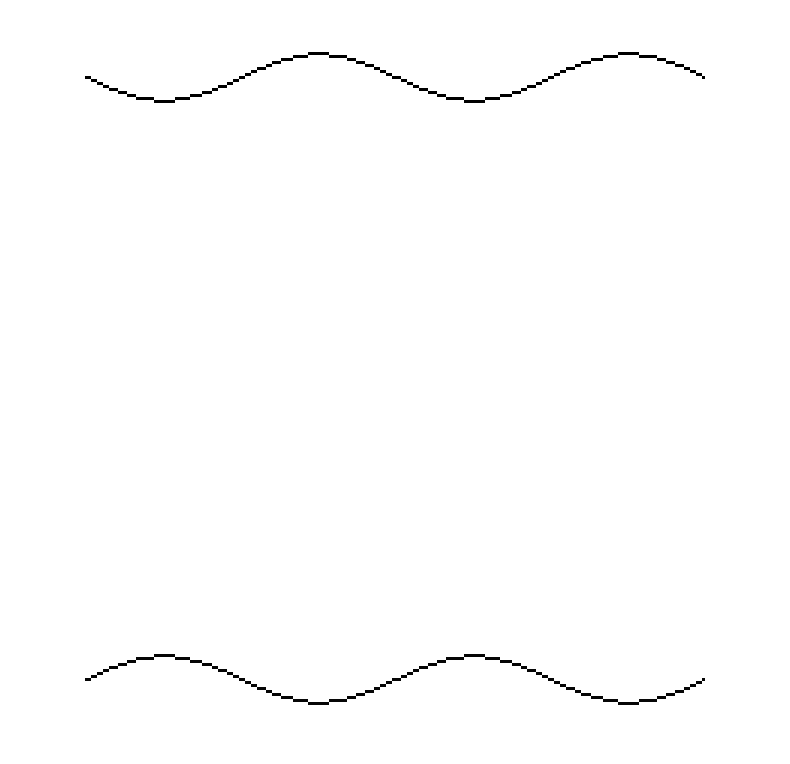
\includegraphics[width=0.155\linewidth]{images/laplacian_analysis/interpolation_space/output_separated_fixed.png} &
        
\includegraphics[width=0.155\linewidth]{images/laplacian_analysis/interpolation_space/output_separated_moving.png} &
        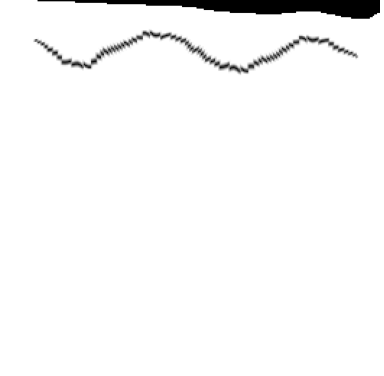
\includegraphics[width=0.155\linewidth]{images/laplacian_analysis/ants/output_image_separate.png} &
        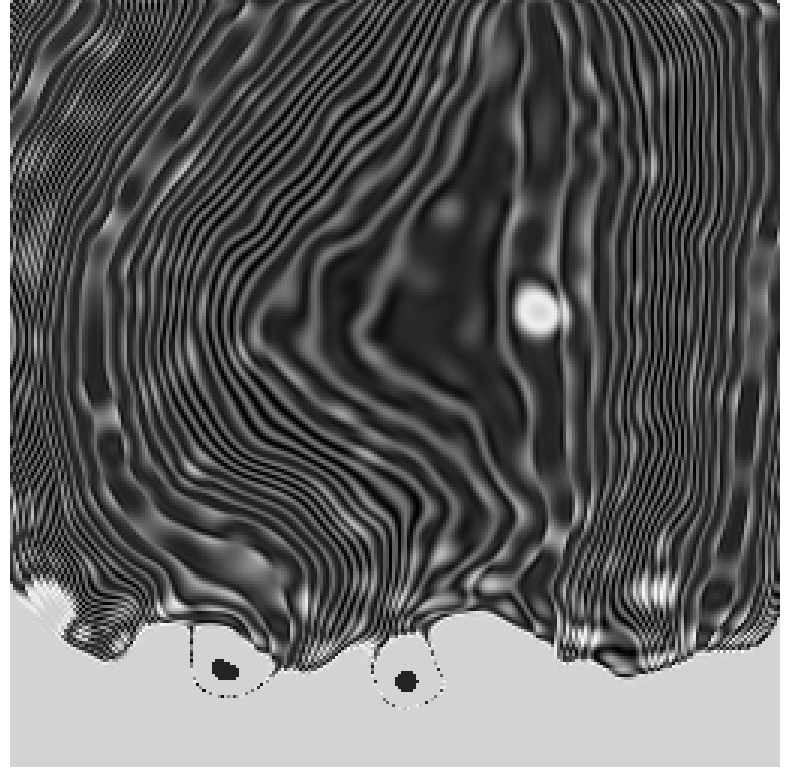
\includegraphics[width=0.155\linewidth]{images/laplacian_analysis/ants/output_elastix_separate.png} \\
        \hline

        % ===== Second row of images =====
        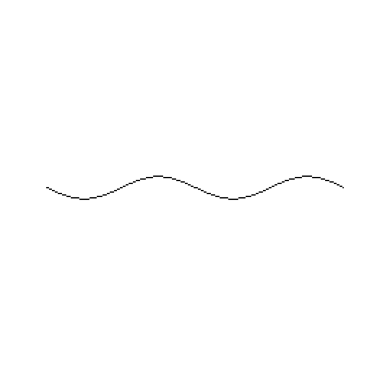
\includegraphics[width=0.155\linewidth]{images/laplacian_analysis/ants/moving_image_helix.png} &
        
\includegraphics[width=0.155\linewidth]{images/laplacian_analysis/ants/fixed_image_helix.png} &
        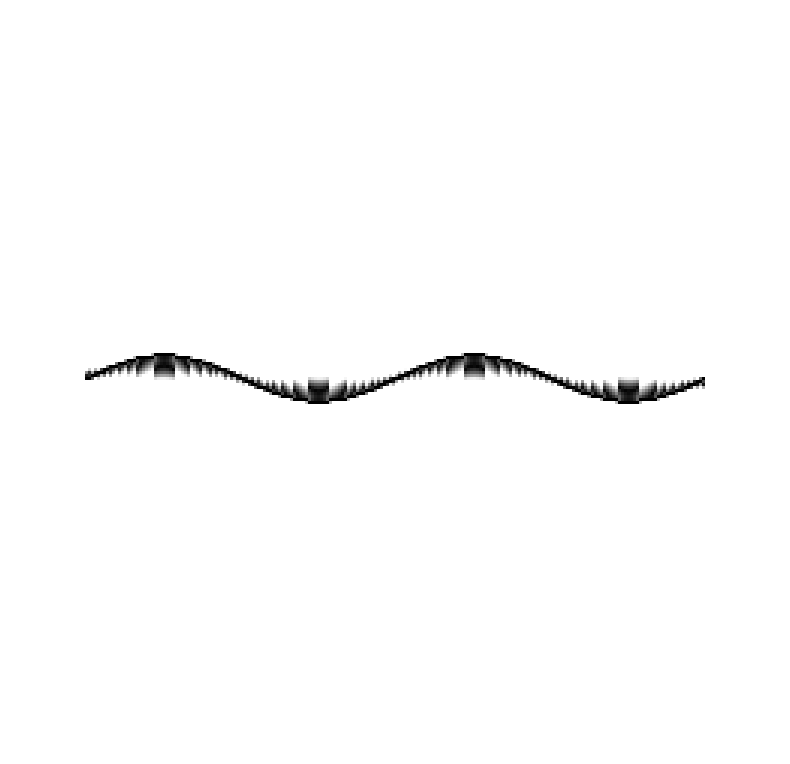
\includegraphics[width=0.155\linewidth]{images/laplacian_analysis/interpolation_space/output_intersecting_fixed.png} &
        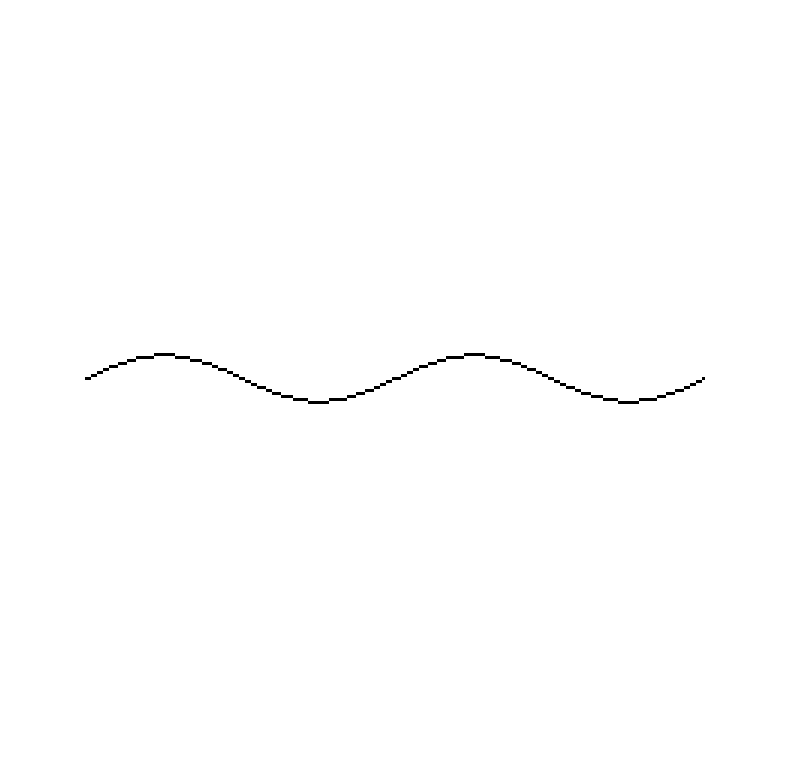
\includegraphics[width=0.155\linewidth]{images/laplacian_analysis/interpolation_space/output_intersecting_moving.png} &
        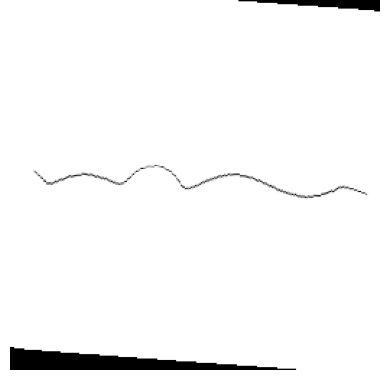
\includegraphics[width=0.155\linewidth]{images/laplacian_analysis/ants/output_image_helix.png} &
        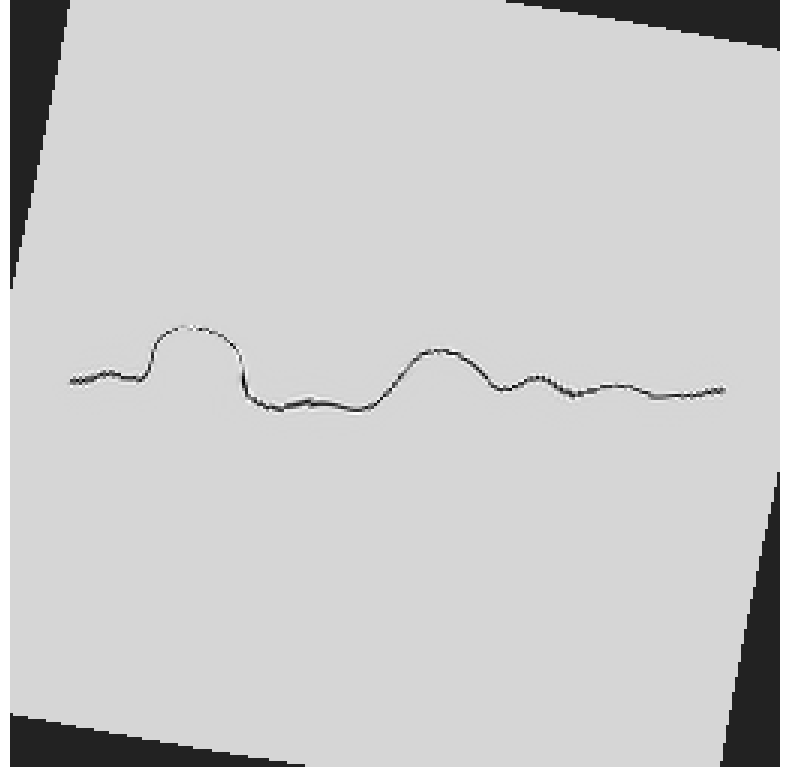
\includegraphics[width=0.155\linewidth]{images/laplacian_analysis/ants/output_elastix_helix.png} \\
        \hline
    \end{tabular}
    \caption{The top row and bottom row show two different experiments. The first column shows the moving image, which must be deformed to register with the fixed image (column 2). The registered output should look exactly like the fixed image. Laplacian interpolation on the fixed image space for registration (using \autoref{eq:dirichlet_boundary_fixed}) shows the duplication artifact (column 3), while Laplacian interpolation on the moving image (column 4) results in a correctly registered image. ANTs (column 5) and Elastix (column 6) show serious artifacts. The second experiment (bottom row) creates a smearing artifact when Laplacian interpolation is done in the fixed image space.}
    \label{fig:fixed_artifacts}
\end{figure*}


\section{Interpolation spaces}
\label{sec:interpolation_spaces}

The first analysis we present is a comparison of Laplacian interpolation in the moving space and in the fixed space.

Using the Dirichlet boundary conditions in the fixed space (\autoref{eq:dirichlet_boundary_fixed}), Laplacian interpolation or any other registration method would give deformation vectors at every pixel in the fixed space that would tell from which pixel in the moving image the output (registered) image would borrow the content (color). Well-known registration techniques such as ANTs \cite{AVANTS200826} and Elastix \cite{Klein2010elastixAT} use interpolation in the fixed space. 

We observe that interpolation in the fixed space will create two problems in the output (registered) image: (1) blurring and smearing artifacts, and (2) duplication of content in the registered image. Both problems can be attributed to many-to-one mappings from the fixed image to the moving image. The third artifact, which is not quite apparent, is that there would be pixels in the moving image that will not have a corresponding point in the fixed image, and so will not contribute anything to the output registered image. This problem arises from the discretization of the computation, which maps only at the pixel centers of the fixed image.

We show these artifacts on a moving and a fixed image whose content is sinusoidal curves with a 180-degree phase difference (see \autoref{fig:fixed_artifacts}). The correspondences between the points on the moving image and the fixed image are apparent — points on the curve on the same vertical line correspond to each other, so every point in the moving image has to either move up or down to register with the fixed image. In the first experimental setup, the curve in the moving image is at the top and the curve in the fixed image is at the bottom, so that all points on the curve in the moving image will move directly down to reach their corresponding point in the fixed image. Based on this movement, all other points in the image would move, and logically, all other points also would move only vertically. In the second setup, both curves are in the center of the image, and these curves intertwine. Although all points in the moving image still move vertically, some points move down and others move up for correct registration with the fixed image curve.

\autoref{fig:fixed_artifacts} shows the results of Laplacian interpolation-based registration in the fixed space and in the moving space, and the results of ANTs and elastix-based registration in these two experimental setups. 

In the first experiment (top row of \autoref{fig:fixed_artifacts}), in the fixed image, vectors are defined on the pixels of the curve towards the location of the corresponding pixels on the curve in the moving image, from where the color has to be fetched. In addition, boundaries of the fixed image will not move, and hence their deformation vectors are set to a zero vector. These form the Dirichlet boundary conditions for interpolation. Deformation vectors for the rest of the pixels in the fixed image will be interpolated from these boundary constraints. The Laplacian interpolation computes a zero vector as deformation vectors for pixels farther from the curve at the bottom and closer to the top edge of the image. In other words, for the pixels closer to the top edge in the fixed image, the color is taken from the same pixel location in the moving image. It so happens that the sinusoidal curve is there in that space in the moving image, and hence in the output (registered) image, that curve is copied (\autoref{fig:fixed_artifacts}, top row, third column). Recall that the points on the bottom curve of the fixed image also received color from this same curve in the moving image. The moving image curve will be referenced twice in the output image, resulting in an incorrect registration image. This artifact is completely eliminated if the corresponding points are defined in the moving image, Laplacian interpolation is done in the moving image space, and the output registered image is composed by taking color from the moving image space. In other words, the boundary condition (initial correspondences) is the only reference to the fixed image space, and the fixed image content is never used. ANTs and Elastix methods also perform interpolation in the fixed image space, and exhibit serious unacceptable artifacts. 

In the second experiment (bottom row of \autoref{fig:fixed_artifacts}) where the sinusoidal curves are in the center of the input images, with Laplacian interpolation in the fixed image space, multiple adjacent pixels in the fixed image that are close to the curve map to the same pixel in the moving image. Thus, the color contribution from the curve in the moving image spreads to multiple pixels in the fixed image, creating a smear. Similar to the first problem, this artifact is also due to many-to-one mappings from the fixed image to the moving image. With interpolation in the moving image, every pixel contributes to only one pixel or its subpixel in the output. So, this smearing problem is completely avoided. Again, ANTs and Elastix produce unacceptable results with the new moving and fixed images.
 

%\textbf{TODO: define the spaces and relation between spaces; define what is good practice}. However, the computation of boundaries in the fixed space is essential for retrieving the mapped points in regions of expansion and compression. 



%Methods that rely on image intensity values, such as ANTs and elastix, may be well-suited for domains with varied and densely populated values, but not for sparsely populated images or images that rely heavily on edge and boundary features, as depicted in \autoref{fig:ants_transformation}. 

\begin{comment}
\begin{figure}
    \centering
    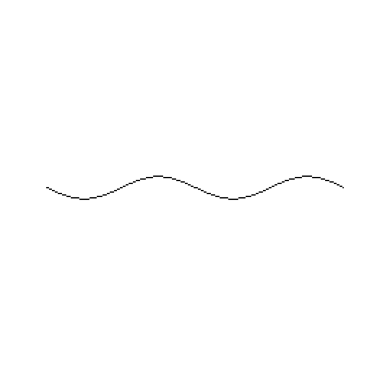
\includegraphics[width=0.24\linewidth]{images/laplacian_analysis/ants/moving_image_helix.png}
    
\includegraphics[width=0.24\linewidth]{images/laplacian_analysis/ants/fixed_image_helix.png}
    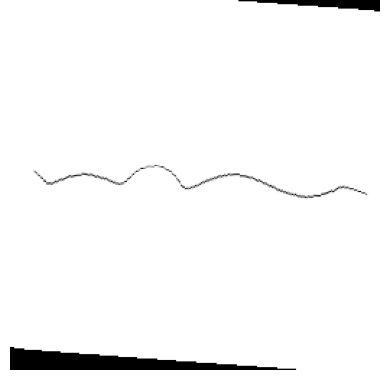
\includegraphics[width=0.24\linewidth]{images/laplacian_analysis/ants/output_image_helix.png}
    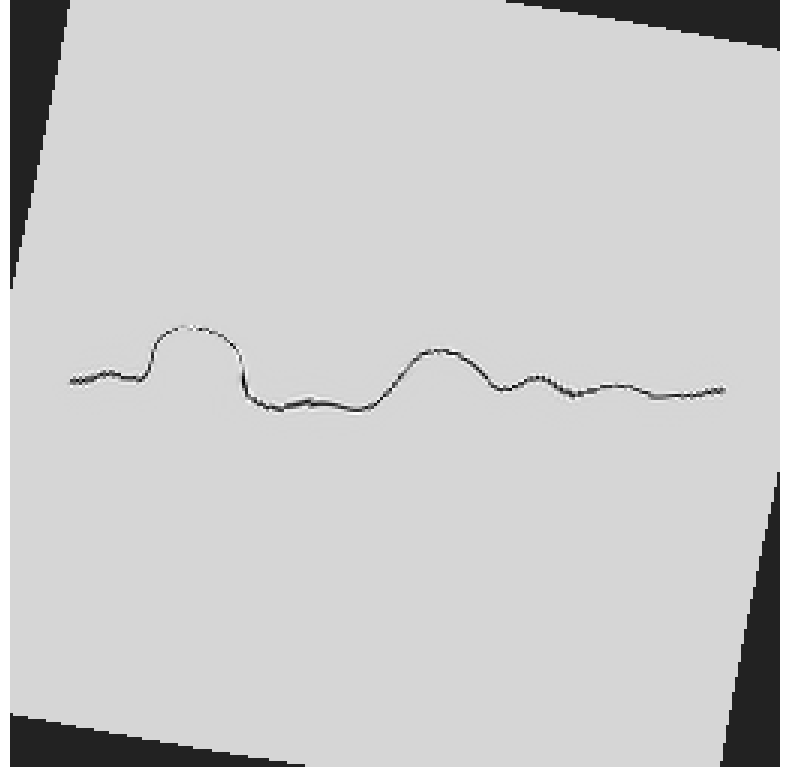
\includegraphics[width=0.24\linewidth]{images/laplacian_analysis/ants/output_elastix_helix.png}
    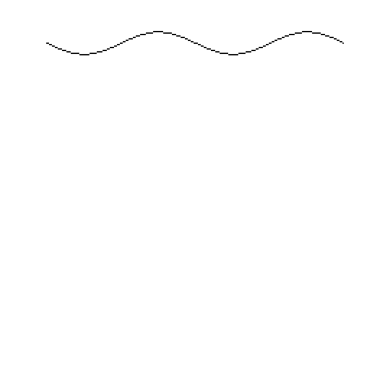
\includegraphics[width=0.24\linewidth]{images/laplacian_analysis/ants/moving_image_separate.png}
    
\includegraphics[width=0.24\linewidth]{images/laplacian_analysis/ants/fixed_image_separate.png}
    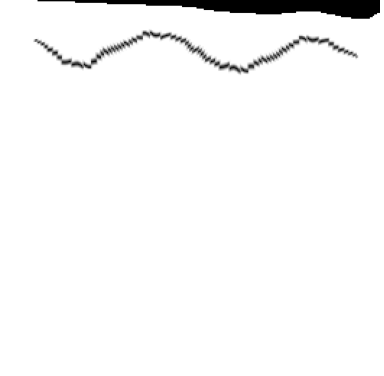
\includegraphics[width=0.24\linewidth]{images/laplacian_analysis/ants/output_image_separate.png}
    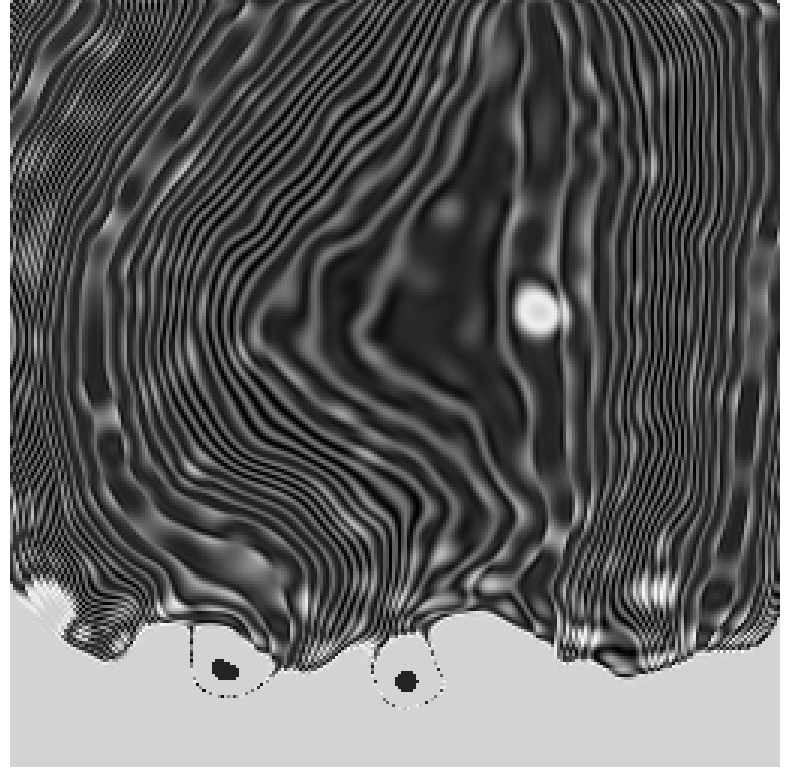
\includegraphics[width=0.24\linewidth]{images/laplacian_analysis/ants/output_elastix_separate.png}
    \caption{A comparison of ANTs SyN and elastix registration run on the correspondences depicted in \autoref{fig:fixed_artifacts}. Though not as prominent as in \autoref{fig:fixed_artifacts}, the registration operation is not well suited for sparsely populated images or images that rely heavily on edge and boundary features.}
    \Description{Two rows of sine wave lines are shown; the first two columns show sine waves, while the third and fourth columns show deformed sine waves.}
    \label{fig:ants_transformation}
\end{figure}
\end{comment}


% SECTION TO EXPLAIN EXPANSION POINT MAPPING
\section{Correspondence augmentation}
\label{sec:new_correspondences}

In the second contribution of this work, we aim to improve the invertibility of the mapping function by reducing the number of points with negative Jacobian determinants after computing a Laplacian interpolation. 

% D1
There are many causes of non-invertibility in mapping. The presented process only reduces the points with non-invertible mappings that are created due to certain numerical errors, especially found in regions of contraction (determinant of Jacobian < 1) and pinching (determinant of Jacobian = 0).

% D1


% D2
 We observe that in regions where the mapping expands the area (Jacobian determinant > 1), adjacent pixels in one image space will map to pixels that are farther than one pixel away in the other image space. Such a mapping is numerically more stable than regions where the mapping compresses the area (Jacobian determinant < 1), where the adjacent pixels are mapped to subpixel coordinates that are closer than a pixel distance away in the other image. In such compressions within a region, minor numerical errors can result in a non-monotonic mapping (see \autoref{fig:mapping_change}) and push the Jacobian determinant to become negative. 

The above observation is within a single image. Let us consider two independent Laplacian interpolations: one in the moving image and the other in the fixed image. We observe that even though the two mappings are independently computed by the two Laplacian interpolations, in general they have an "inverse" behavior — the regions of contraction from the moving image map to the regions of expansion in the fixed image, and vice versa (\autoref{fig:correspondences}). However, the exact correspondences computed for moving image pixels and those computed for fixed image pixels using the above two independent Laplacian operations are {\em not} inverses of each other. This particular property provides us with the necessary new information to address some of the numerical errors. 

The core idea to reduce the numerical error issue that leads to the reduction of points with negative Jacobian determinants is the following. The regions of compression mapping in the moving image can borrow the correspondences imposed by the corresponding regions of the expansion mapping in the fixed image. However, the two mappings (using, say, Laplacian interpolations) have to be independently calculated, as we described earlier. Using these observations, we present the following algorithm.

\begin{comment}
Specifically, we focus on adjacent pixels in the moving image space that get mapped to subpixels of the same or very close pixels in the fixed image space. An important observation to note is that between image spaces, there is an \textbf{inverse behavioral property} such that regions in the moving image space experience a contraction of area in the fixed image space under the computed mapping. Conversely, the mapping from the fixed image space to the moving image space in those same regions experiences an expansion of area (see \autoref{fig:correspondences}). 
\end{comment}

%However, as previously noted, they contain an inverse behavioral property such that expansion in one image space corresponds with contraction in the other space, and vice versa. 


% D2
We first compute the Laplacian interpolation in the fixed image space, using which, we compute the corresponding points of all the fixed image pixels in the moving image. Then we compute the Jacobian determinant for all pixels in the fixed image using \autoref{eq:central_differences}. 

%Although these Jacobian determinant values are computed on two independent Laplacian interpolations in two different spaces, we observe that the Jacobian determinant of > 1 in one space correlates with the Jacobian determinant of < 1 in its corresponding region in the other image space. 

We define $t$ ($t>1$) as a threshold for a Jacobian determinant value above which the particular pixel in the fixed image will be considered to have an expanding mapping in the moving image. For all fixed image pixels $p_f$ with Jacobian determinant > t, we find their corresponding mapped point $map(p_f)$ in the moving space and set their correspondences to point to itself ($map(map(p_f))=p_f$).
Finally, the updated correspondence list for the moving image, along with the original set of correspondences, are used as new Dirichlet conditions for the Laplacian interpolation on the moving image. These results in a mapping from moving image to fixed image with improved diffeomorphic properties.
These additional correspondences do not affect the visual fidelity of the registration operation (see \autoref{fig:real_data_sections}) as the changes are done only to the regions in the moving image that undergo contraction under this mapping. 

%To reduce folding artifacts and improve invertibility in the registration field, we update the initial set of point correspondences by identifying regions of local expansion (where the Jacobian determinant is large) and interpolating new correspondences based on the upsampled deformation field.


%We note that when computing the Jacobian determinants for the deformations in the moving and fixed spaces, the Jacobian determinant values for both reflect vertically across the middle of the grid, as seen in \autoref{fig:correspondences}. 
 
%Though updating these refined correspondences does not guarantee that instances of negative Jacobian determinants are eliminated, we observe that the number of non-positive Jacobians decreases across our experiments. 


\begin{figure}
    \centering
    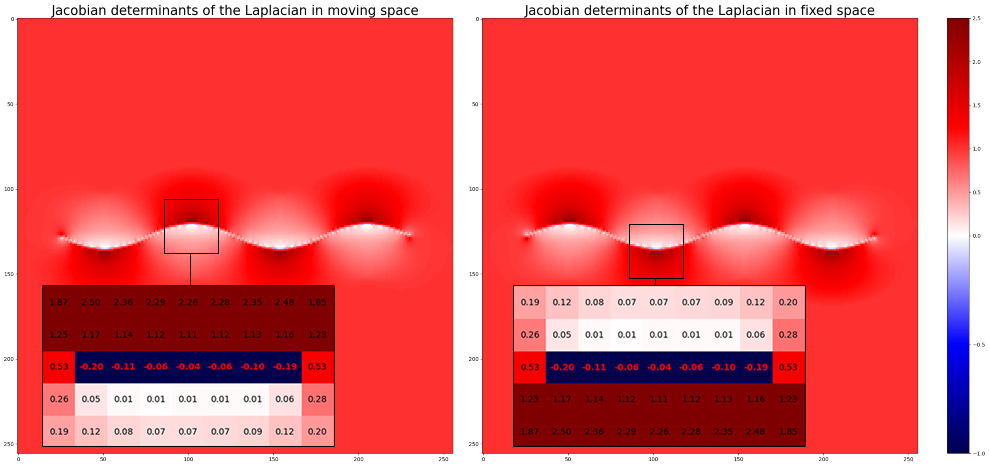
\includegraphics[width=\linewidth]{images/laplacian_analysis/initial_correspondences.png}
    \caption{We showcase the output of a Laplacian operation on a set of sinusoidal moving/fixed correspondence points taken from the second row of \autoref{fig:fixed_artifacts}. The Jacobian determinant values are depicted in the interpolated moving (left) and fixed space (right). The close-up zoom-in window depicts regions of interest in both spaces and the Jacobian determinant value in each pixel. In general, >1 Jacobian determinant regions in one image are mapped to <1 Jacobian determinant regions in the other image and vice-versa. Our algorithm has to focus on such regions where this relationship is exhibited, and not on regions that are close to input correspondences or pixels with Jacobian determinants very close to 1.0, where this relationship may not be strictly or consistently observed.}
    \label{fig:correspondences}
\end{figure}

The following is the step-by-step description of the process.

Let $D': \Omega' \rightarrow \mathbb{R}$ denote the Jacobian determinant field over the fixed image domain $\Omega'$, and let $\phi': \Omega' \rightarrow \mathbb{R}^2$ be the deformation vector field. 
Let $$\Psi: \Omega' \rightarrow \Omega, \quad \Psi(x) = x + \phi'(x), \quad \forall x \in \Omega'$$ be the coordinate mapping such that coordinates in the fixed image $\Omega'$ are mapped to coordinates in the moving image $\Omega$.
%Let $m$ be a function that maps coordinates in $\Omega'$ to coordinates in $\Omega$, such that $m(x_1, x_2) = (x_1, x_2) + \phi'(x_1, x_2)$ for all $(x_1, x_2) \in \Omega'$. 
We identify the expanding regions in $\Omega'$ by thresholding the Jacobian determinant:
    $$
        \mathcal{E} = \left\{ (x_1, x_2) \in \Omega' \;\middle|\; D'(x_1, x_2) > t \right\},
    $$
    where $t>1$ is a user-defined threshold (e.g., $t = 1.3$). 
    %Jacobian determinant values greater than 1.0 denote regions of $\Omega'$ that stretch/expand in the mapped region in $\Omega$. 

% D3
From the coordinates in $\mathcal{E}$, we add the new correspondences, 
$$\left(\Psi(x), x\right), \quad x \in \mathcal{E},$$
to the moving image as additional Dirichlet boundary conditions and compute Laplacian interpolation on the moving image with these new boundary conditions. This updated image deformation of $\Omega$ reduces the numerical errors and thus significantly reduces regions with negative Jacobian determinants.

There is an implementation detail that needs to be taken care of in the above algorithm. The coordinate mapping $\Psi(x)$, where $x\in \mathcal{E} $, need not result in integer coordinates in $\Omega$. However, to introduce it as a boundary condition, $\Psi(x)$ has to be an integer coordinate, and $x$ may have floating point coordinates. Just rounding off $\Psi(x)$ will introduce numerical errors, so we find the subpixel coordinates in $\Omega'$ around $x$ whose mapping is closest to $round(\Psi(x))$. This can be achieved to a reasonable precision by upscaling $\Omega'$ and bilinearly interpolating the $\Psi(x)$ function in the upscaled $\Omega'$.
\begin{comment}
    We define the following steps:

\begin{enumerate}
    \item \textbf{Upsample the coordinate mapping} $\Psi$ by a factor $s=3$ using bilinear interpolation. To preserve consistency, original displacements are enforced at aligned grid locations:
    $$
        \Psi^{\uparrow}(sx_1, sx_2) = \Psi(x_1, x_2), \quad \forall (x_1, x_2) \in \Omega'.
    $$

    \item \textbf{Identify expanding regions} by thresholding the Jacobian determinant:
    $$
        \mathcal{E} = \left\{ (x_1, x_2) \in \Omega' \;\middle|\; J'(x_1, x_2) > t \right\},
    $$
    where $t$ is a user-defined threshold (e.g., $t = 1.1$). Jacobian determinant values greater than 1.0 denote regions of $\Omega'$ that stretch/expand in the mapped region in $\Omega$. These are the regions that are less likely to cause folding. 
    
    \item \textbf{For each expanding coordinate} $(x_1, x_2) \in \mathcal{E}$:
    \begin{itemize}
        \item Evaluate the upsampled coordinate mapping $\Psi^{\uparrow}$ at:
        $$
        \Psi^{\uparrow}(sx_1, sx_2),
        \quad 
        \Psi^{\uparrow}(sx_1 \pm 1, sx_2),
        $$
        $$
        \Psi^{\uparrow}(sx_1, sx_2 \pm 1),
        \quad
        \Psi^{\uparrow}(sx_1\pm1, sx_2 \pm  1).
        $$
        
        \item Retrieve the corresponding displaced (mapped) locations:
        $$
        %y_i = (x_1, x_2) + \phi'^{\uparrow}(p_i), 
        y_i = \Psi(p_i)
        \quad \text{for `} p_i \in \text{neighbor coordinates}.
        $$
        
        \item Select the $y_i$ that is closest to the rounded integer central grid location:
        $$
        y^\ast = \arg\min_{y_i} \| y_i - \text{round}(\Psi^{\uparrow}(sx_1, sx_2)) \|.
        $$
        
        \item Record a new correspondence:
        $$
        \text{Fixed point: } f = (x_1, x_2), \quad \text{Moving point: } m = y^\ast.
        $$
    \end{itemize}
    
    \item \textbf{Postprocess} to remove any:
    \begin{itemize}
        \item Duplicates in $(m, f)$ pairings.
        \item Points that overlap with previously assigned correspondences.
    \end{itemize}
    
    \item \textbf{Combine} the new pairs $\{(m_i, f_i)\}$ to the original correspondence set:
    $$
    C_m \leftarrow C_m \cup \{m_i\}, \quad
    C_f \leftarrow C_f \cup \{f_i\}.
    $$

    \item \textbf{Re-run Laplacian interpolation} using the new set of correspondences $C_m$ and $C_f$.
\end{enumerate}

\end{comment}


% D2
\begin{comment}
Although the Laplacian operation can be performed in either moving or fixed space to retrieve a deformation, it is best practice to perform it in moving space due to numerous factors in application.
In these transformations, retrieving and applying a deformation in fixed space using the boundary conditions in \autoref{eq:dirichlet_boundary_fixed} ensures that every pixel in the fixed space contains a displacement vector, mapping each pixel in the fixed space to a corresponding pixel coordinate in the moving space.
In contrast, using \autoref{eq:dirichlet_boundary_moving} ensures that each pixel in the moving space has a displacement vector that determines its position in the moving space.
\end{comment}
\begin{figure}
    \centering
    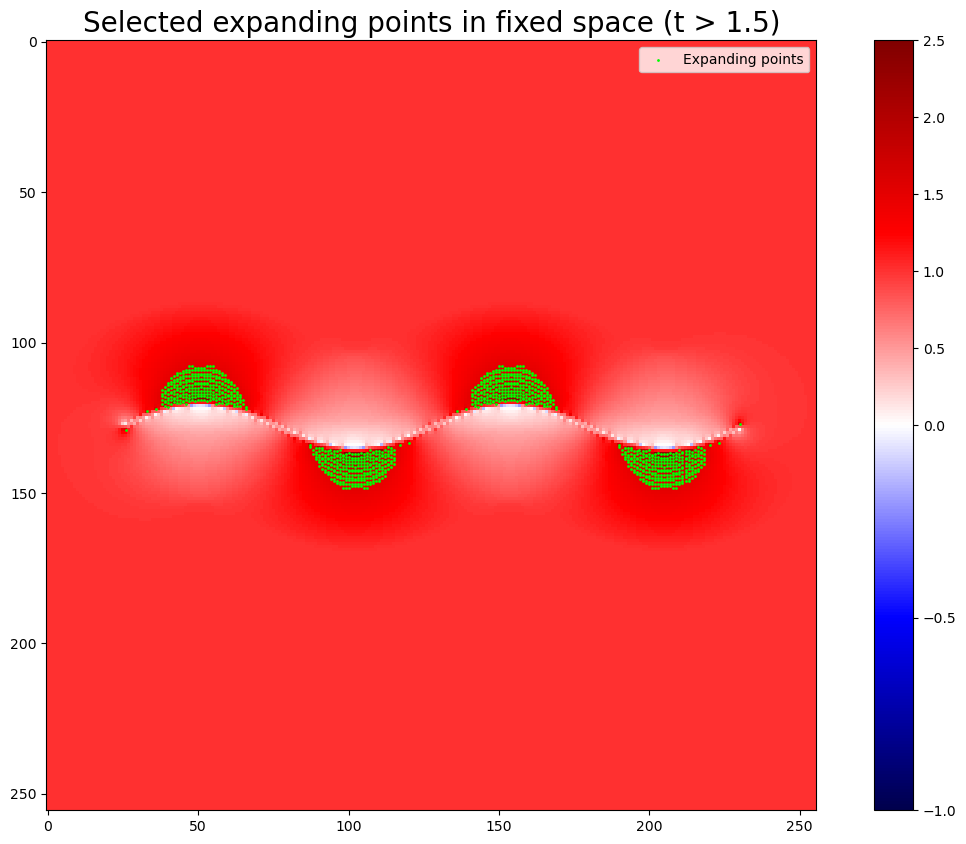
\includegraphics[width=0.49\linewidth]{images/laplacian_analysis/expanding_points_1.5.png}
    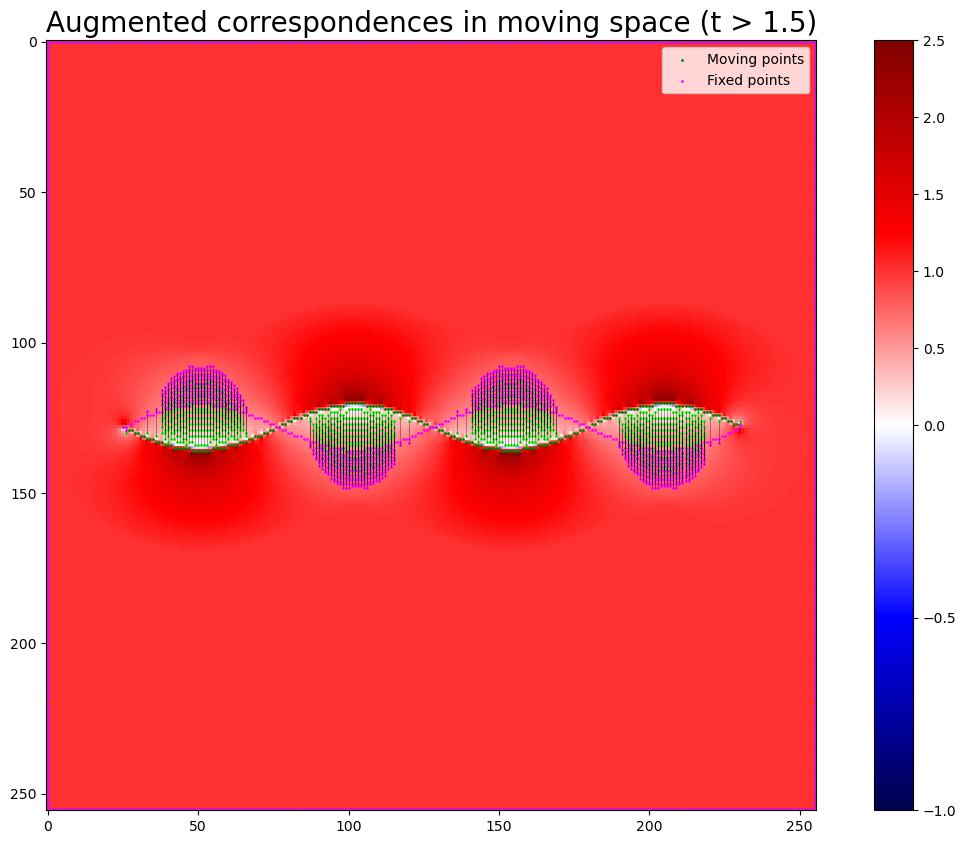
\includegraphics[width=0.49\linewidth]{images/laplacian_analysis/augmented_points_1.5.png}
    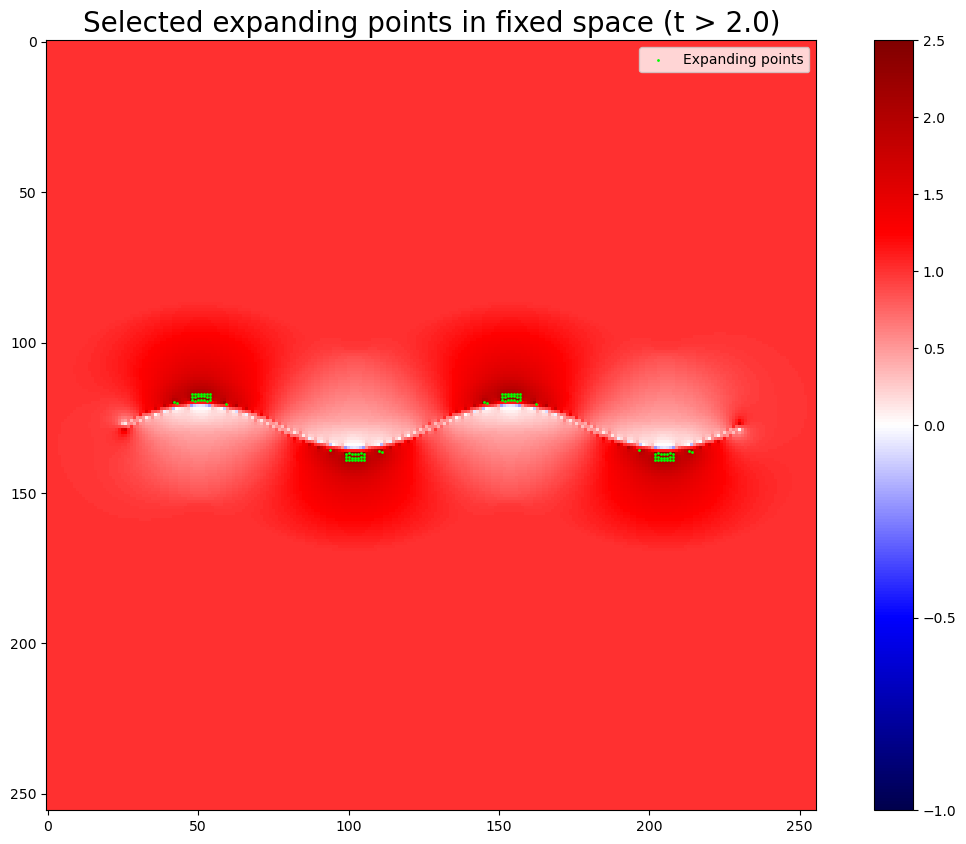
\includegraphics[width=0.49\linewidth]{images/laplacian_analysis/expanding_points_2.0.png}
    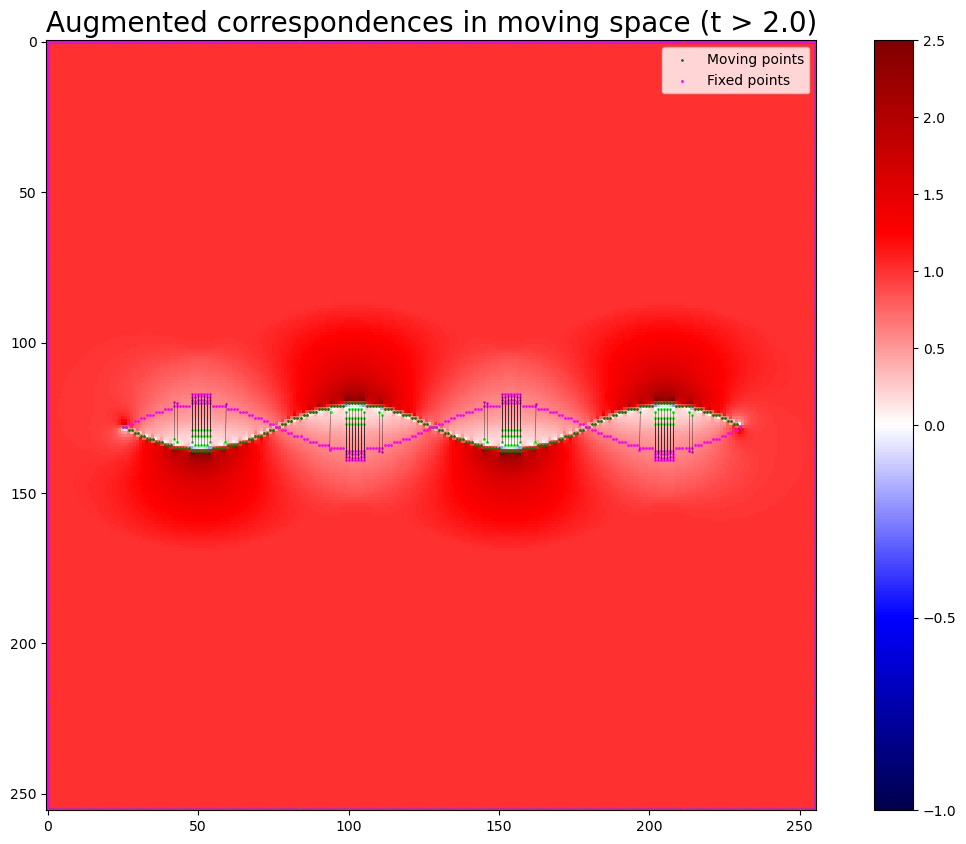
\includegraphics[width=0.49\linewidth]{images/laplacian_analysis/augmented_points_2.0.png}
    \caption{New correspondences added using $t$ > 1.5 (first row) and $t$ > 2.0 (second row). The newly added correspondences are depicted in green and magenta. We observe that for $t$ > 2.0, the number of non-positive Jacobian determinants has changed from 52 to 28, or in the case of $t$ > 1.5, have all positive Jacobian determinants.}
    \label{fig:new_correspondences}
\end{figure}

% D3
By using existing information about the original set of correspondences, we avoid introducing conflicting correspondence information and fine-tune the original deformation field further to better correct instances of folding, as seen in \autoref{fig:mapping_change}.

\begin{figure}
    \centering
    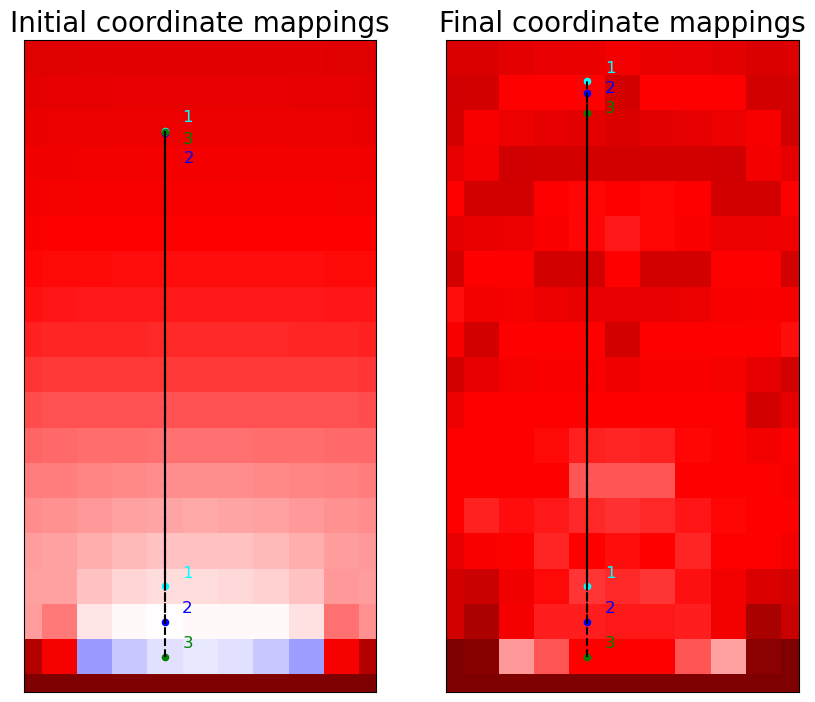
\includegraphics[width=\linewidth]{images/laplacian_analysis/mapping_change.png}
    \caption{New mappings (right) are generated from the initial Laplacian run on the left, generated from the points in the bottom row of \autoref{fig:fixed_artifacts} and as seen in \autoref{fig:correspondences}, where the sinusoidal waves intersect with each other and are mapped only in the vertical direction. In this coordinate mapping, the coordinates are plotted such that the coordinates on the bottom (moving points) map to the coordinates on the top (fixed points) with respect to their labeled numbers (e.g. point 1 is mapped to point 1, point 2 is mapped to point 2, etc.). Blue pixels indicate negative Jacobian determinant values and instances of folding. To prevent folding, the coordinate mappings should be monotonic. However, on the left, the bottom-most coordinate 3 is mapped to the middle-most coordinate on the top. This out-of-sequence mapping is due to numerical errors, as deformation is only done vertically in this case. On the right, after running with the new augmented correspondences, the correspondences and folding are now corrected, showing that the bottom-most coordinate 3 is now mapped to the bottom-most coordinate on the top.}
    \label{fig:mapping_change}
\end{figure}

We apply and observe the results of refining correspondences across our test cases and on sets of correspondences retrieved from real mouse brain data from \cite{RegBoost2025, TexeraMouseBrain} in \autoref{tab:results} and \autoref{fig:real_data_sections}. 

\begin{comment}
\begin{figure}
    \centering
    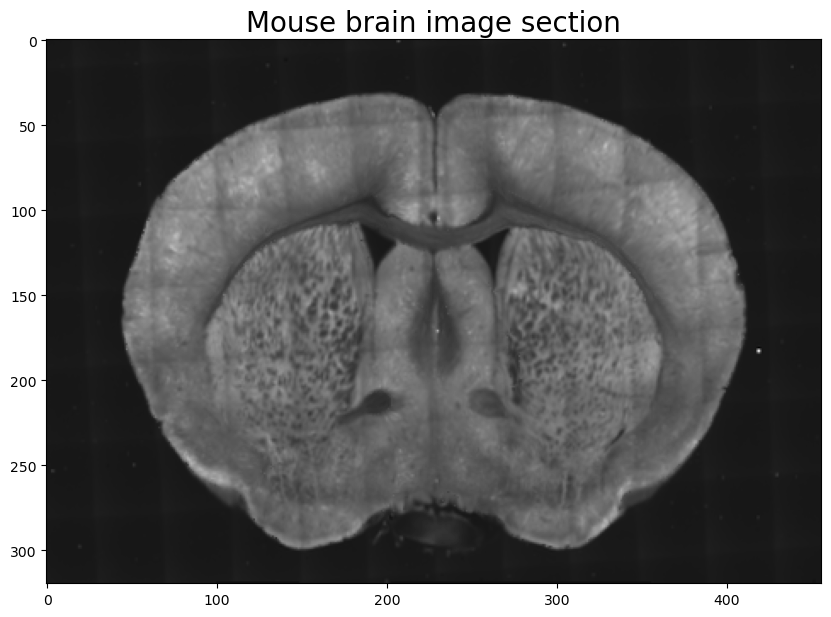
\includegraphics[width=0.49\linewidth]{images/laplacian_analysis/mouse_brain/mouse_brain_input.png}
    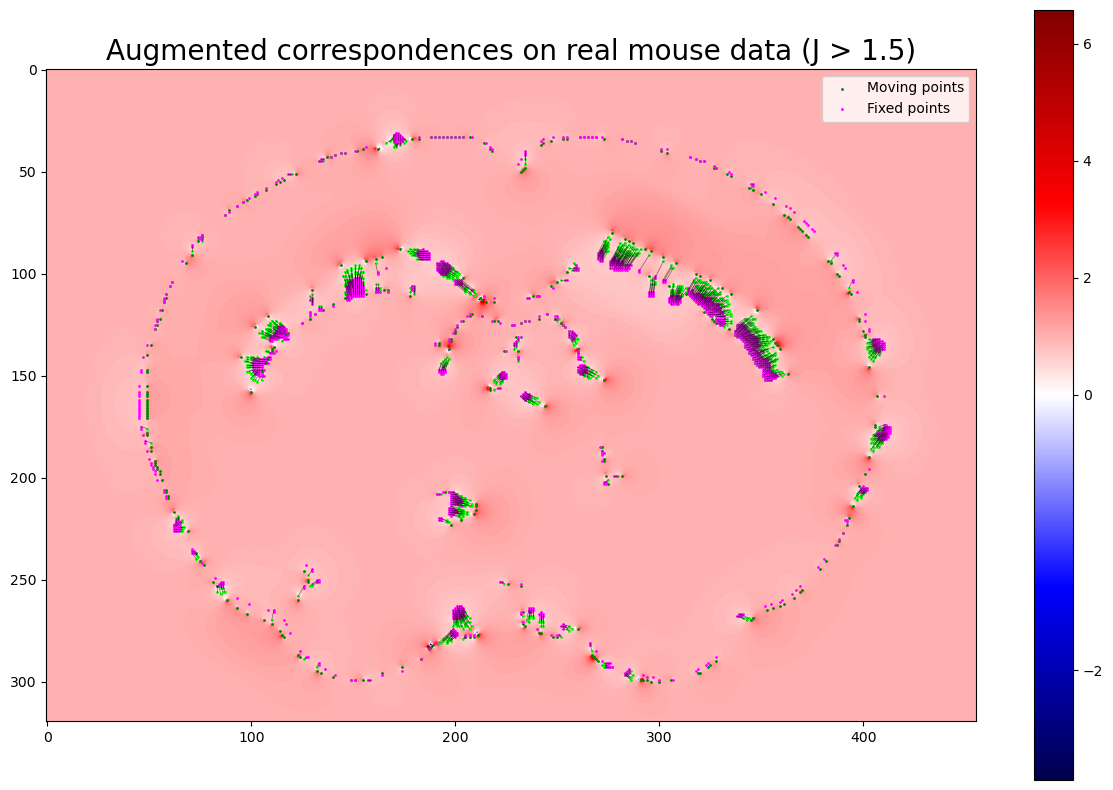
\includegraphics[width=0.49\linewidth]{images/laplacian_analysis/mouse_brain/augmented_correspondences_200.png}
    \caption{The following method applied on correspondences retrieved from real mouse brain data. On the left, the initial mouse brain section is shown. On the right, the augmented correspondences (connected by lines from moving green points to fixed purple points) with $t$ > 1.5 are shown with the Jacobian determinant values, with a minimum Jacobian determinant of -2.80 and 29 non-positive Jacobian determinants from its original -1.61 and 61.}
    \Description{A microscopic mouse brain section is shown, along with a plot of points corresponding to features and edges in the mouse brain.}
    \label{fig:real_data}
\end{figure}
\end{comment}

\begin{table}[ht]
    \caption{We run our method on correspondences from synthetic and real data. In our results, we find that introducing our methodology to Laplacian interpolation will reduce the occurrences of non-positive Jacobian determinant valued regions. We present results run on varying $t$ thresholds, and without our correspondence augmentation method.}
    \label{tab:results}
    \begin{tabular}{lccccc}
    \toprule
    Data & $t$ & $\det{(J_r)} \le 0$ \\
    \hline
    Sinusoidal waves 1 & w/o augmentation & 52 \\ % minj = -0.20, maxj = 2.50
    Sinusoidal waves 1 & 2.0 & 30 \\ % minj = -0.15, maxj = 2.63
    Sinusoidal waves 1 & 1.5 & 0 \\  % minj = 0.18, maxj = 2.89
    Sinusoidal waves 1 & 1.3 & 0 \\  % minj = 0.18, maxj = 3.03
    \hline
    Sinusoidal waves 2 & w/o augmentation & 5783 \\ % minj = -1.93, maxj = 7.27
    Sinusoidal waves 2 & 2.0 & 288 \\ % minj = -0.55, maxj = 13.38s
    Sinusoidal waves 2 & 1.5 & 220 \\  % minj = -0.55, maxj = 13.67
    Sinusoidal waves 2 & 1.3 & 186 \\  % minj = -0.49, maxj = 14.04
    \hline
    Mouse brain section 1 & w/o augmentation & 63  \\ % section 200, minj = -3.51, maxj = 6.16
    Mouse brain section 1 & 2.0 & 33  \\ % section 200, minj = -2.75, maxj = 6.47
    Mouse brain section 1 & 1.5 & 27 \\  % section 200, minj = -2.78, maxj = 6.58
    Mouse brain section 1 & 1.3 & 26 \\  % section 200, minj = -2.78, maxj = 6.52
    \hline
    Mouse brain section 2 & w/o augmentation & 56  \\ % section 350, minj = -1.99, maxj = 4.21
    Mouse brain section 2 & 2.0 & 34  \\ % section 350, minj = -1.78, maxj = 4.24 
    Mouse brain section 2 & 1.5 & 25 \\  % section 350, minj = -1.71, maxj = 4.14
    Mouse brain section 2 & 1.3 & 21 \\ % section 350, minj = -1.59, maxj = 4.01
    \hline
    Mouse brain section 3 & w/o augmentation & 71  \\ % section 500, minj = -2.74, maxj = 5.21
    Mouse brain section 3 & 2.0 & 35  \\ % section 500, minj = -1.81, maxj = 4.98
    Mouse brain section 3 & 1.5 & 29 \\ % section 500, minj = -1.83, maxj = 4.95
    Mouse brain section 3 & 1.3 & 27 \\ % section 500, minj = -1.91, maxj = 5.03 
    \bottomrule
    \end{tabular}
\end{table}

\begin{figure*}[ht]
    \centering
    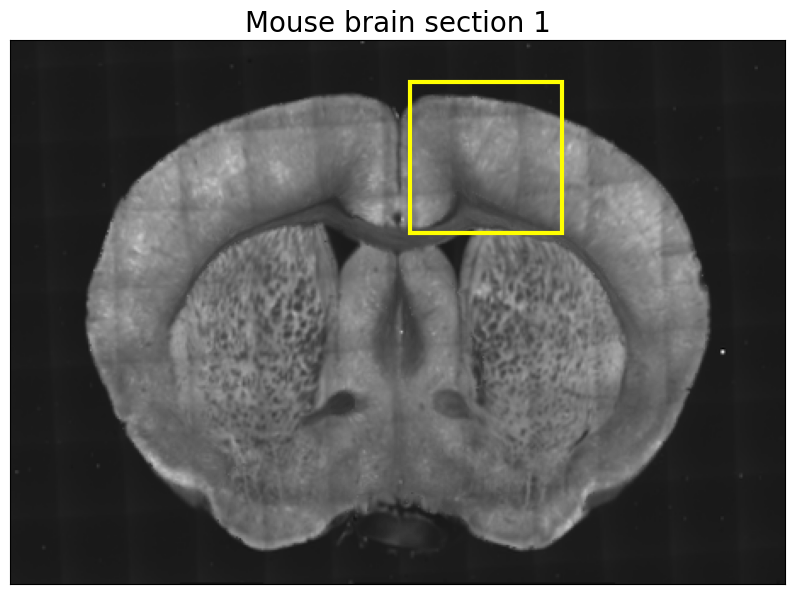
\includegraphics[width=0.33\linewidth]{images/laplacian_analysis/mouse_brain/mouse_brain_1.png}
    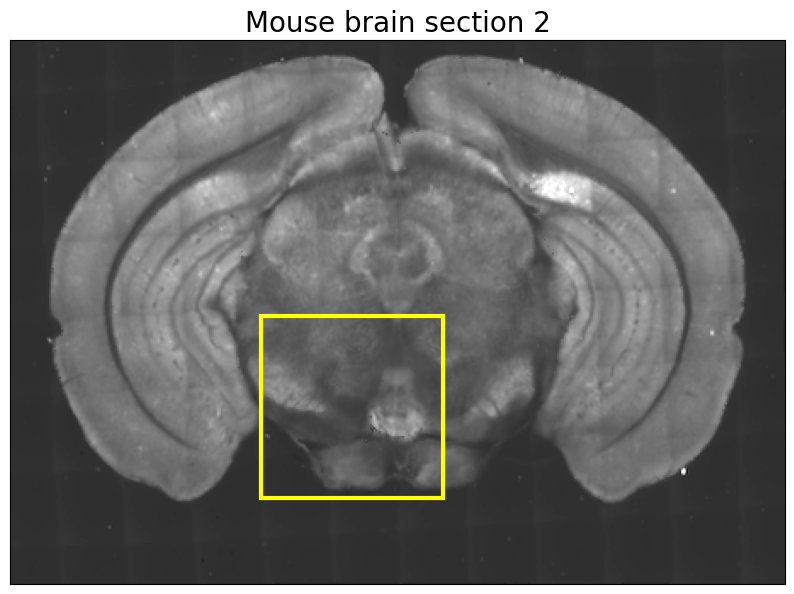
\includegraphics[width=0.33\linewidth]{images/laplacian_analysis/mouse_brain/mouse_brain_2.png}
    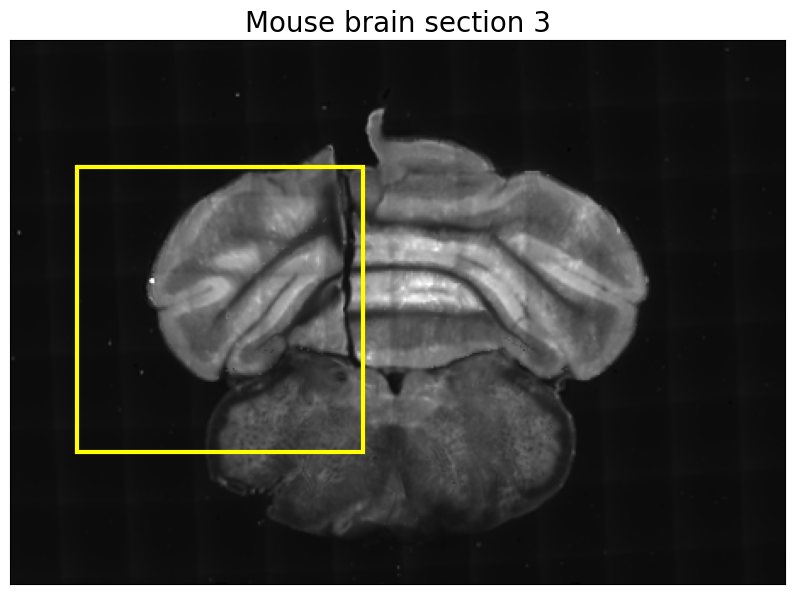
\includegraphics[width=0.33\linewidth]{images/laplacian_analysis/mouse_brain/mouse_brain_3.png}

    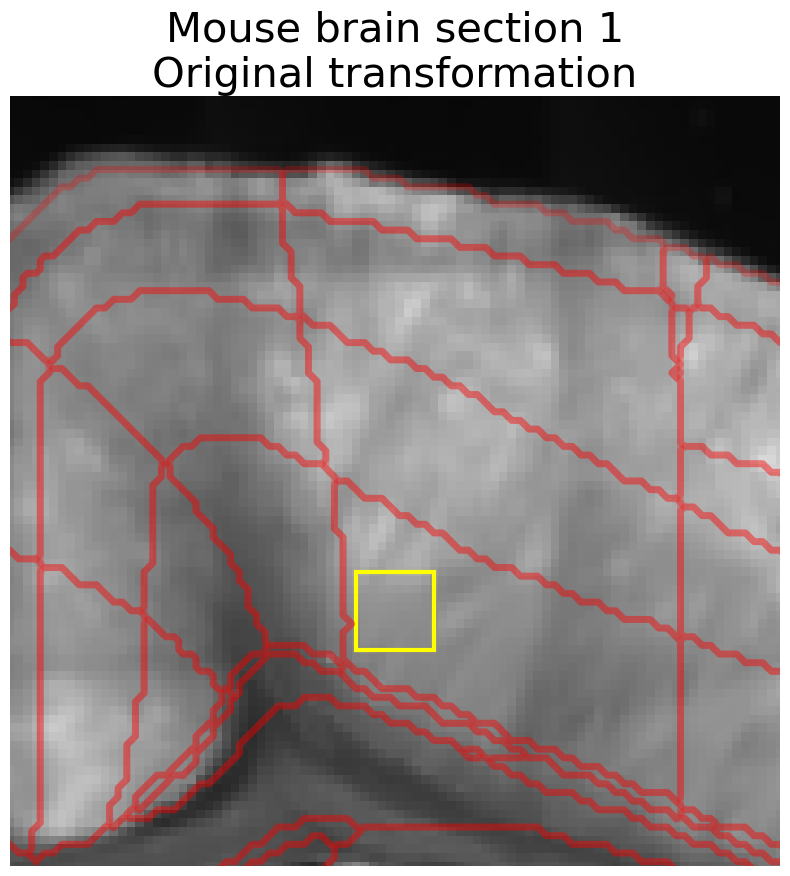
\includegraphics[width=0.16\linewidth]{images/laplacian_analysis/mouse_brain/mouse_brain_1_before_real.png}
    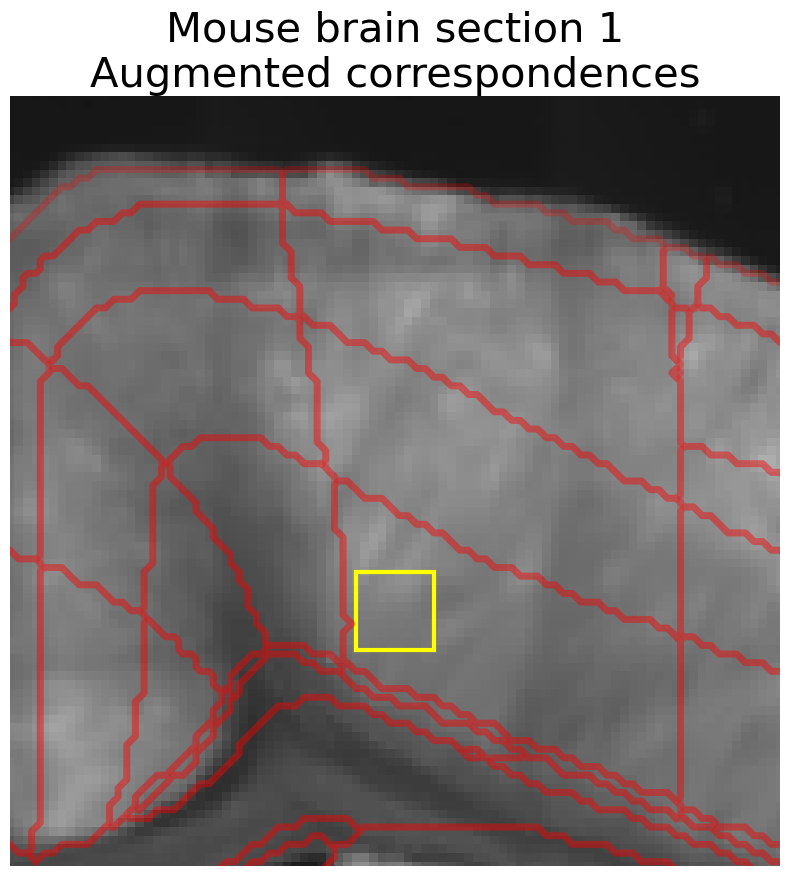
\includegraphics[width=0.16\linewidth]{images/laplacian_analysis/mouse_brain/mouse_brain_1_after_real.png}
    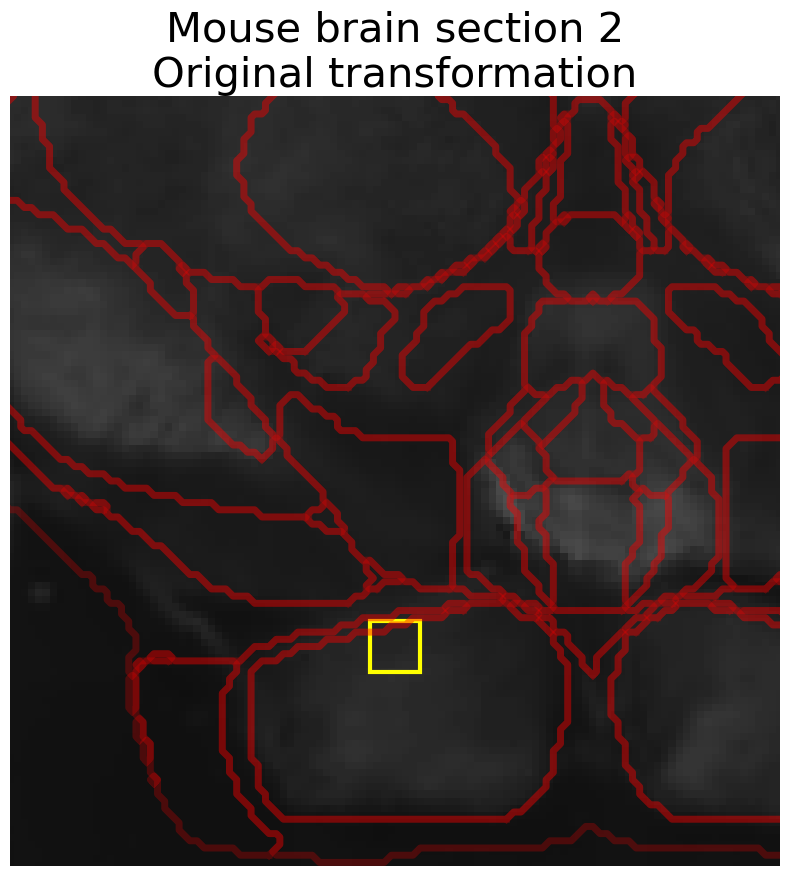
\includegraphics[width=0.16\linewidth]{images/laplacian_analysis/mouse_brain/mouse_brain_2_before_real.png}
    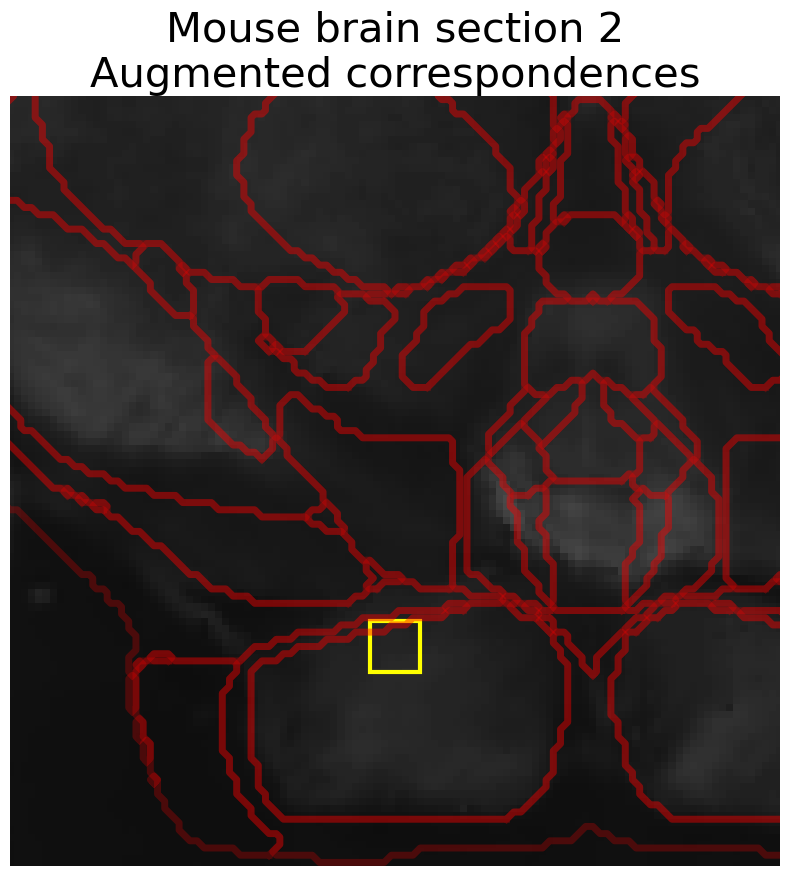
\includegraphics[width=0.16\linewidth]{images/laplacian_analysis/mouse_brain/mouse_brain_2_after_real.png}
    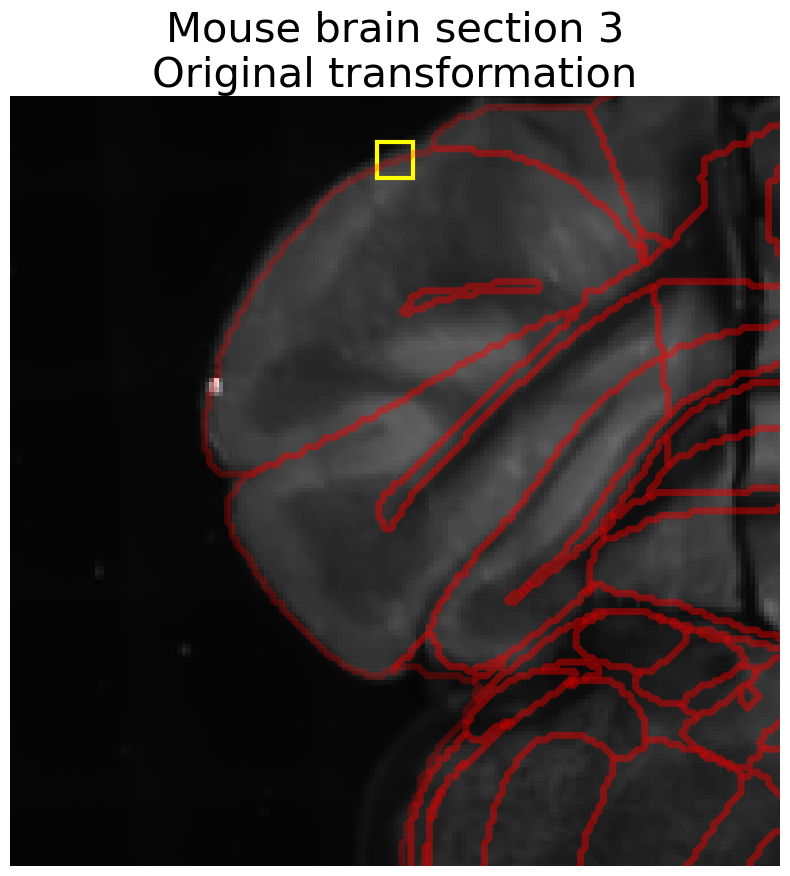
\includegraphics[width=0.16\linewidth]{images/laplacian_analysis/mouse_brain/mouse_brain_3_before_real.png}
    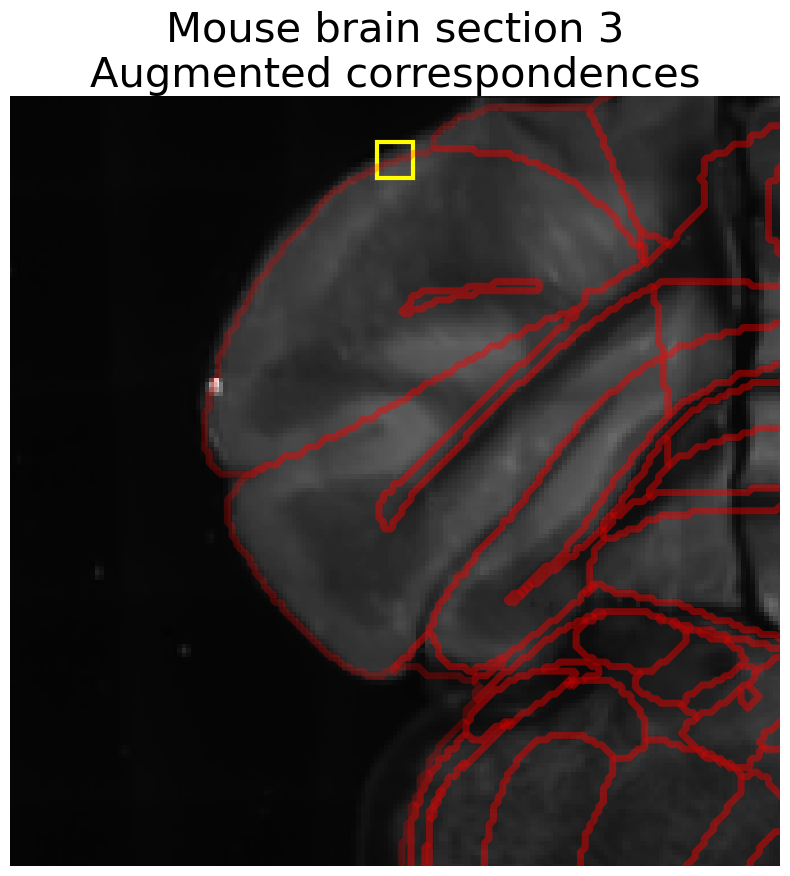
\includegraphics[width=0.16\linewidth]{images/laplacian_analysis/mouse_brain/mouse_brain_3_after_real.png}
    
    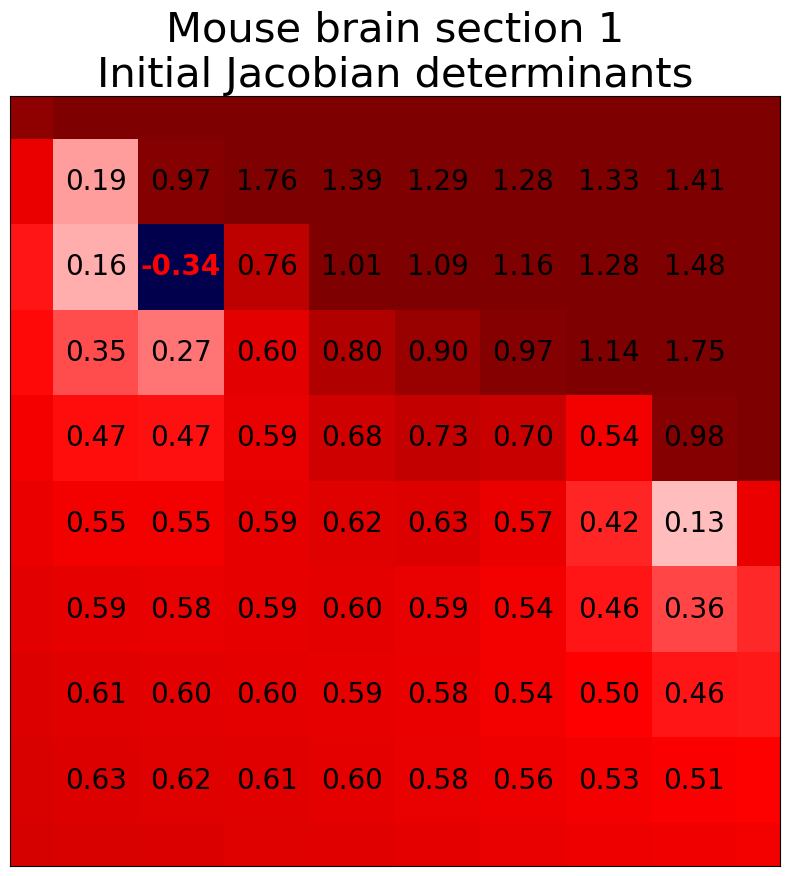
\includegraphics[width=0.16\linewidth]{images/laplacian_analysis/mouse_brain/mouse_brain_1_before_jdet.png}
    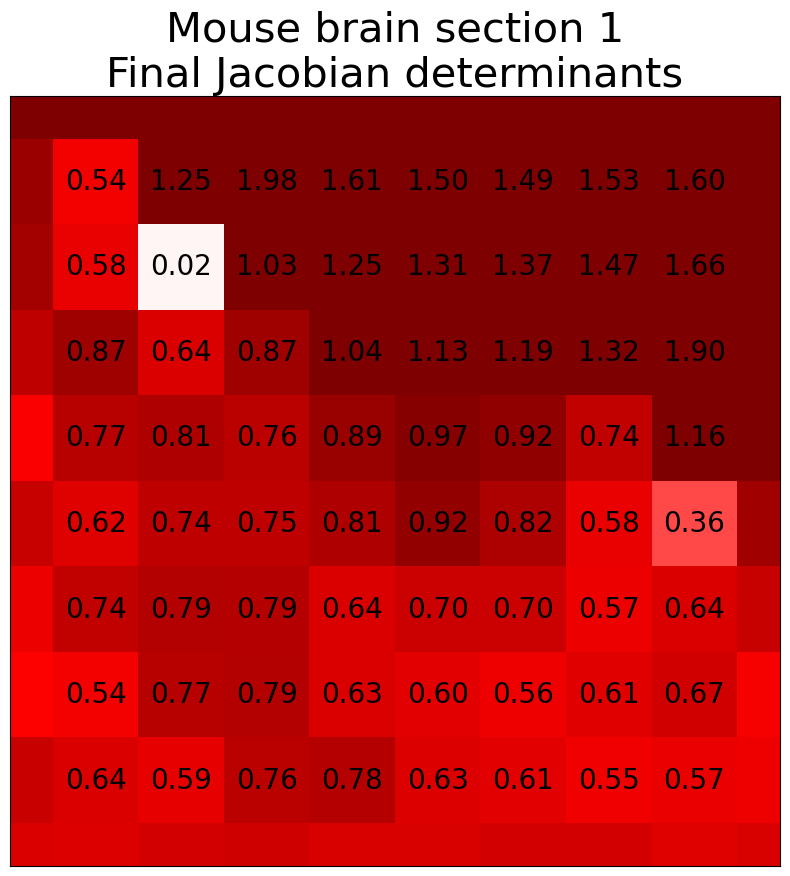
\includegraphics[width=0.16\linewidth]{images/laplacian_analysis/mouse_brain/mouse_brain_1_after_jdet.png}
    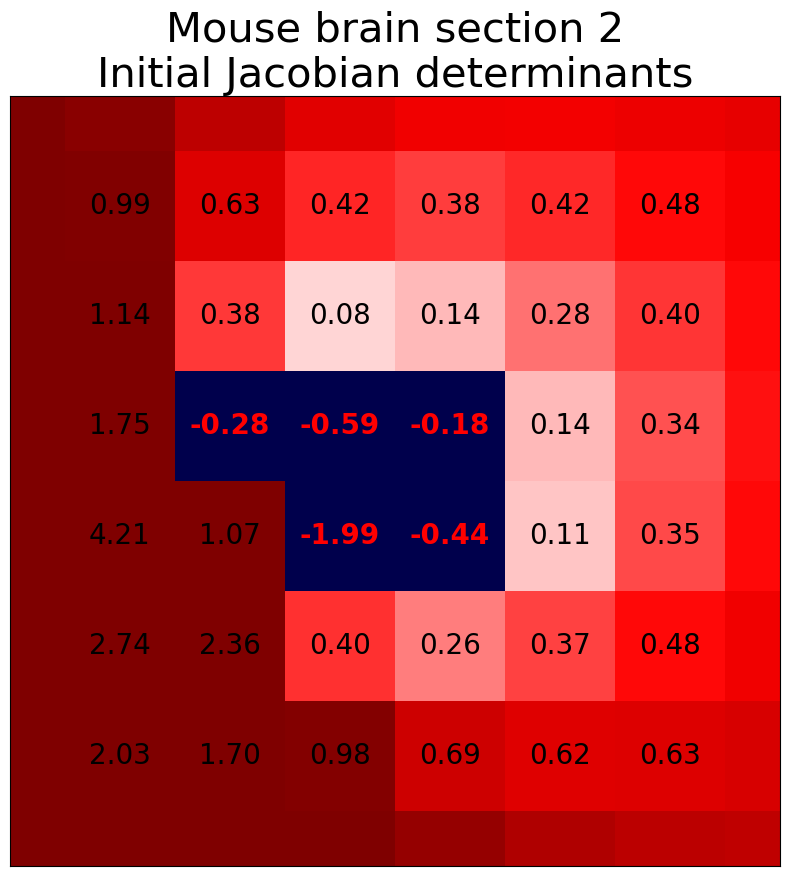
\includegraphics[width=0.16\linewidth]{images/laplacian_analysis/mouse_brain/mouse_brain_2_before_jdet.png}
    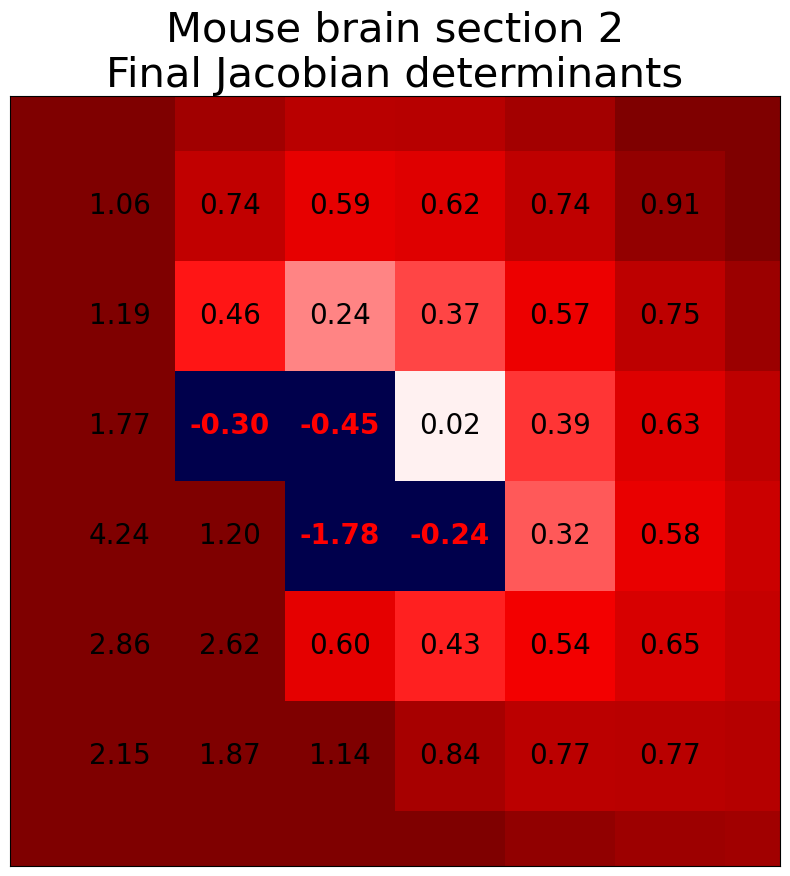
\includegraphics[width=0.16\linewidth]{images/laplacian_analysis/mouse_brain/mouse_brain_2_after_jdet.png}
    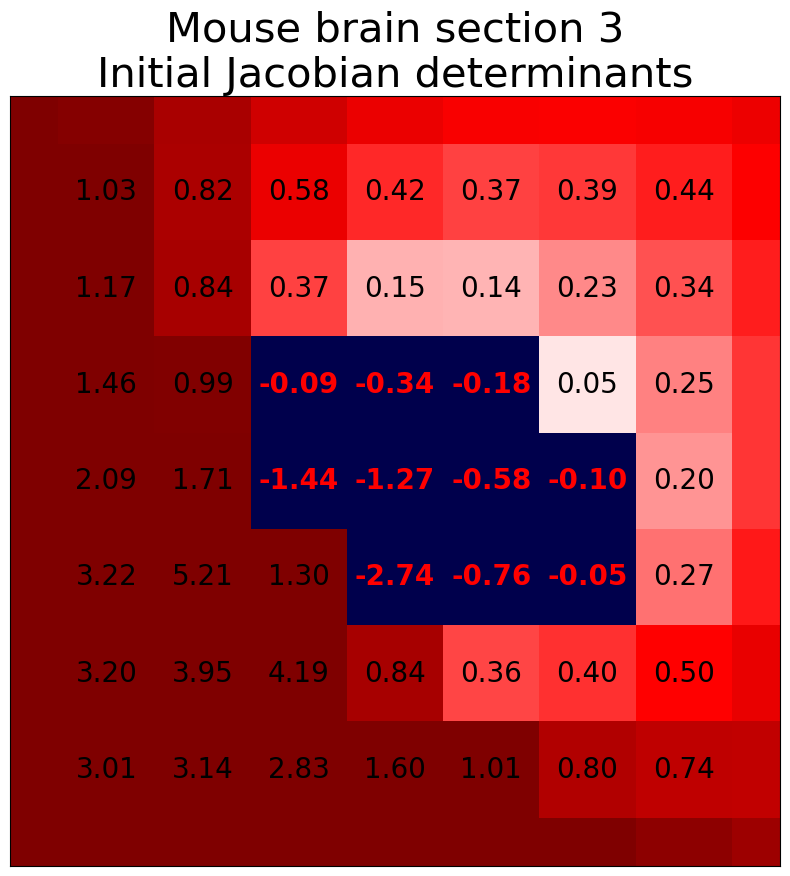
\includegraphics[width=0.16\linewidth]{images/laplacian_analysis/mouse_brain/mouse_brain_3_before_jdet.png}
    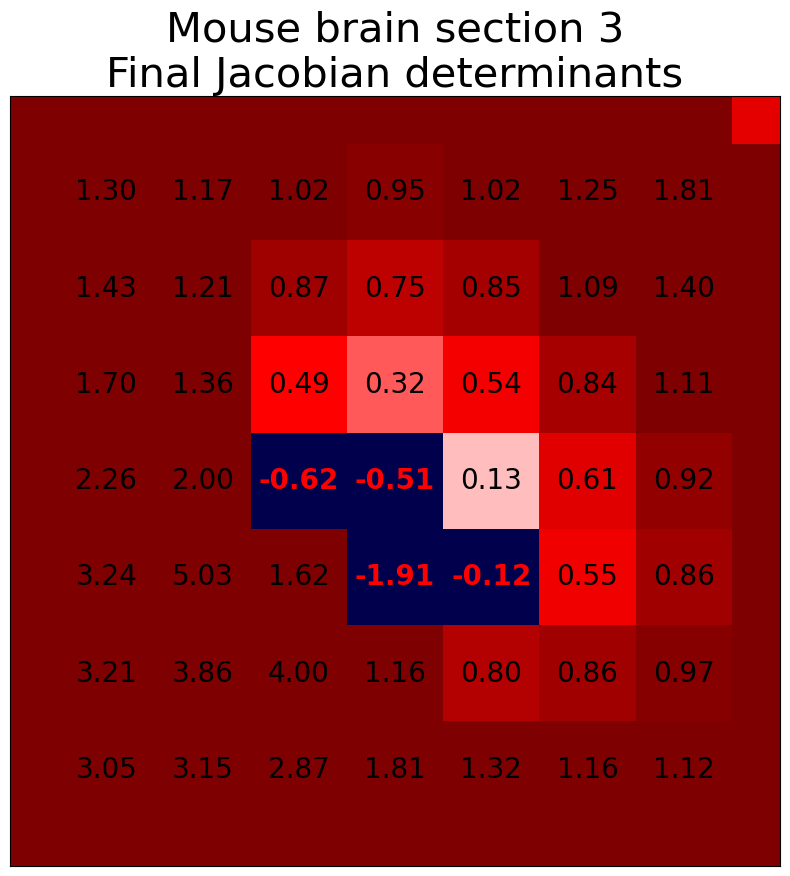
\includegraphics[width=0.16\linewidth]{images/laplacian_analysis/mouse_brain/mouse_brain_3_after_jdet.png}
    \caption{Mouse brain sections 1, 2, and 3 from \autoref{tab:results} are shown in the first row from left to right. Their transformations before and after using the augmented correspondences are depicted in the second row in the regions from the boxed windows in the first row. The resultant images do not undergo any changes in visual fidelity; however, their underlying deformation vectors are more invertible due to changes at the subpixel level. The third row indicates regions of improvement in the boxed windows from the second row, before and after augmenting the correspondences.}
    \label{fig:real_data_sections}
\end{figure*}

All code and implementations used for these experiments are uploaded and made publicly available at <redacted>.

\section{Conclusion}

In this study, we propose the best practice in interpolation space for registering two images: When a moving image has to be warped to register with a fixed image, current popular methods perform inverse warping of the fixed image and reconstruct the output image by "texture mapping" (taking color values from) the moving image. We show that this approach can lead to artifacts in the registration image such as displacement blurring and feature duplication, especially in areas of compression or sparse correspondence support. We further show that computing the deformation function in the moving image removes these artifacts and produces better registration quality than traditional approaches. 

In the second contribution, we analyze the limitations of Laplacian interpolation for image registration, particularly concerning local invertibility as measured by Jacobian determinant values. To mitigate these problems, we introduced a framework based on augmenting the correspondences for the moving image, by borrowing them from the displacements computed on the fixed image. By identifying regions of local expansion using the Jacobian determinant, we generated new correspondences through subpixel interpolation, improving the overall quality of the estimated deformation field.

Our results demonstrate that updating and augmenting correspondences using this strategy significantly reduces the number of negative Jacobian determinants and enhances the invertibility of the registration. 

Future work will explore integrating this method into existing registration algorithms, and extending it to three-dimensional datasets with real anatomical variability. Additionally, another venue for exploration would be to study how noisy correspondences (e.g., automatically detected correspondences) can affect the Jacobian determinant values and the number of non-positive Jacobian determinants, assuming that not all correspondences may reflect the ground truth. Lastly, better metrics for understanding folding may provide insight into better understanding and fully resolving occurrences of non-positive Jacobian determinants. Current methods of computing Jacobian determinants to represent local deformation in discretized grids utilize information from points adjacent to each pixel of interest, excluding the information inherent in the pixel of interest itself. Though the exclusion of the current pixel coordinate can be rectified with finite differences, not all of the values of its neighbors will be accounted for. This can lead to potential misclassifications of regions with folding in edge cases that may be affected by numerical approximation. Metrics that take into account changes in triangulation between corresponding points may yield future insight into optimizing for fully diffeomorphic outputs. 





\begin{abstract}
Deformable image registration is a fundamental computational technique used in many biomedical applications. These methods function by aligning an input image data set with a template image by moving every pixel of the input image to register with the corresponding pixel in the template image. The collection of these vectors defined over the pixels of the input image for alignment with the template image, is called a deformation vector field (DVF).

% These registration operations output transformations, which are modeled through deformation vector fields (DVFs). 
    
% For many such registration applications, ensuring good alignment and accuracy to the template image is sufficient. However, for analyses directly involving DVFs, 

It may be necessary to ensure that the transformations defined by the DVFs are smooth, invertible, and free of folding artifacts. 
%DVFs that do not fulfill these conditions can introduce topological deformations that are anatomically impossible. 
Not all registration methods guarantee smooth and invertible transformations. Although there have been various methods to reduce the number of these folding artifacts during the registration process, little work has been done to process and modify existing DVF outputs to eliminate folding. 
    
In this paper, given a DVF that is computed using any preferred method, we present a framework to process and ensure local invertibility of the input DVF while minimizing deviation from the input DVF.  The presented work is efficient, fast, and parallelizable,  and makes minimum changes to the input DVF to make it invertible.  

\end{abstract}






\section{Introduction}
\label{sec:introduction}

Image registration is a critical process in many computational biomedical workflows. Researchers and clinical experts commonly utilize image registration methods to align images and data, potentially from different modalities or specimens, into a common standardized or shared reference frame. This registration process maps pixels of one image (moving image) to another (fixed image), and this mapping is encoded as deformation vectors at every pixel of the moving image, which when added to the moving image's pixel coordinate will give the mapped fixed image's pixel coordinate. The collection of these displacement vectors is called the deformation vector field (DVF).
\begin{comment}
and subsequent alignment is achieved by retrieving and identifying corresponding features between pairs of moving (input) and fixed (template) images, which is then used to spatially map data from one image space to another. The result is a transformed version of the moving image, deformed to fit to the fixed image features and space, using deformation vector fields (DVFs) that define where each pixel or voxel within the images is to be shifted.
\end{comment}
\begin{comment}
% save for bigger journal:
These deformations are indispensable in many real-world applications, particularly when utilized alongside atlases. While organ atlases are commonly known to be used as references to study anatomy in the context of education \cite{GloyAnatomyAtlas, VoxelMan}, they play an important role in research work regarding registration. Specifically, these atlases can be used as reference volumes to establish a standardized frame to align to \cite{CABEZAS2011e158}. Notable examples include the Allen Mouse Brain Common Coordinate Framework \cite{WANG2020936}, the Waxholm Space atlas \cite{Waxholm2023}, the Visible Human Project \cite{VisibleHumanProject}, and the Human Reference Atlas \cite{HumanReferenceAtlas}. 

These atlases typically consist of single volumetric images, often constructed as averaged volumes from multiple specimens. These volumes may come with segmentation masks for key anatomical sub-regions. In registration workflows, these averaged volumes act as the fixed template images. Deforming moving image inputs to these templates allows all specimens deformed to the atlas to lie in the same standardized reference space for effortless analysis, as the segmentation masks that accompany the atlases can be used to identify, compare, or semantically segment anatomical regions of interest, assuming the volumes are sufficiently well-aligned \cite{AtlasSegmentationReview, MultiatlasSegmentation}. 

Image registration is not limited to just aligning data to templates; it can also be performed between two sets of images. In clinical applications, registration allows for scans of patients taken from different time-steps to be aligned and analyzed together in longitudinal studies. Standardizing and deforming images to account for changes in volume due to issues such as breathing artifacts and tissue growth between scans can be critical for identifying and analyzing health metrics such as measurement of lung failure \cite{Reinhardt2008-ty} and tumor mass effects \cite{Zacharaki2009-xu}.
\end{comment}

For many of these deformations, accuracy of registration is the most important criterion. %\cite{WELLS199635, Maes1997-lg, Pluim2003-ha} 
\cite{SENGUPTA2022174, CZOLBE2023102830, HEINRICH20121423}. 
Even if the mapping is not bijective, if it is not injective then the moving image "folds" on the fixed image, leading to anatomically impossible alignments. 
%Although in many cases, the registration may also require a bijective mapping. In some cases, the output transformed image can look accurate to the template, but the underlying deformation field used to achieve this transformation may not be topologically feasible, resulting in anatomically impossible operations to align the data that stem from points in the DVF that "fold" onto each other. 
This can be avoided by ensuring local invertibility, which guarantees that the mapping between the source and target images is smooth and one-to-one within a neighborhood around each point. %This preserves spatial coherence and prevents pathological deformations such as folding or tearing occurring that will result in a non-diffeomorphic transformation. 

Locally invertible deformation vector field is particularly critical in applications such as medical imaging, where the integrity of anatomical structures must be maintained to support reliable analysis, diagnosis, and treatment planning, and hence is the major motivating factor for the presented work. 
% This is especially so in applications involving analysis of data containing 3D or 4D time-step dimensions, as these displacement values can be retrieved for longitudinal analysis such as measuring changes in lung capacity \cite{LungTissueExpansion, Bhatt2017-mp, DeepLearningElasticCT} and rates of swelling in traumatic brain injuries \cite{Cole2018-jc, SNA42}. 


We present a framework for minimally modifying a deformation vector field to make it locally invertible. We propose computationally efficient methods to correct such non-invertible folding artifacts. Furthermore, we demonstrate how our methods can be applied to enhance future work in registration algorithms.

\subsection{Main contributions}
\label{subsec:main_contributions}

Our main contributions can be summarized as follows:

\textbf{Deformation Vector Field processing}: We introduce our method for processing deformation vector field on images that is flexible and can be appended as a module to any 2D registration framework.

\begin{comment}
\textbf{Analysis of causes of non-invertibility}: We define folding artifacts and analyze factors that can lead to folding in registration and the subsequent deformation vector fields. 

\textbf{Eliminating folding and ensuring local invertibility}: We present a method to process existing deformation fields, identifying sub-regions within the deformation that contain local folding artifacts, and modifying the displacement vectors in these regions by applying constraints in an optimizer. The result outputs a new deformation field that adheres to local invertibility constraints and differs minimally from the original deformation field. This method is fast, parallelizable, and does not require additional computation of any registration process during iteration; we demonstrate the robustness of this method and analyze its accuracy.
\end{comment}

\textbf{Local invertibility:} We present a quadratic programming based method that ensures local invertibility of a 2D deformation vector field by guaranteeing positive Jacobian determinant at all points while minimizing deviation from the input deformation vector field.

\textbf{Efficient processing:} We also present a  method that makes the entire 2D deformation field processing more efficient with dramatically reduced run-time, while maintaining the desired accuracy. This method is fast, robust, and parallelizable and does not require additional computation from any registration process.  

Our research offers a comprehensive and automated framework that can process 2D deformation vector fields in such a way that guarantees that these outputs are locally invertible, while minimizing the deviation from the input deformation vector field. We also explore potential directions for further research in this field. 


\section{Related work}
\label{sec:related_work}

%Many registration methods have been developed throughout the history of modern computing, and the list of methods grows each year, boasting increasingly better performance and runtime speed and benefits and drawbacks; 
Registration methods, especially in the biomedical image literature, have a long history, and many review papers offer an in-depth overview of these developments \cite{KLEIN2009786}. 

\textbf{Rigid registration.}
Rigid registration in medical image alignment is comprised of only translation and rotation operations without any scaling or deformation. The use cases assume that the anatomical structures of interest remain unchanged in shape and size across images, making it suitable for scenarios such as inter-subject alignment with minimal structural changes.

\begin{comment}
Classical registration methods typically rely on optimizing similarity measures between moving and fixed images. Such metrics like mutual information \cite{WELLS199635, Viola1997}, sum of squared differences \cite{Khosravi2018}, and cross-correlation \cite{Lewis1994, Stefano2003} are widely used alongside optimization techniques, which can range from gradient descent to multi-resolution and stochastic approaches \cite{MAINTZ19981}. Mutual information in particular has proven particularly effective for multi-modal registration (e.g., CT to MRI), as it captures statistical dependence between intensities in different imaging modalities \cite{Tagare2015}.

Though comparatively simple relative to its other options, rigid registration remains effective and relevant, and it provides invertible transforms.
\end{comment}

Rigid transformation provides invertible transforms and can especially be used as a preprocessing step for more complex non-rigid transformations or for learning-based methods, serving as initial coarse alignment for subsequent fine-grained deformation models \cite{Frackowiak2004-yy}. For 3D data, transformation using point clouds to minimize point distances, such as the Iterative Closest Point (ICP) algorithm %\cite{Besl1992}
\cite{Zhang1994IterativePM}, can be used alongside other models.

\textbf{Non-rigid registration:}
More complex registration methods use pixel/voxel-wise intensity comparisons to accomplish more complicated non-rigid transformations. These methods aim to maximize similarity measures and energy functionals without requiring any explicit feature extraction or landmark identification \cite{regreviewsong}. Regularization terms are typically added to the energy functionals  to constrain smoothness and discourage folding or unrealistic warping \cite{Reithmeir2024}. This makes intensity-based registration highly generalizable and suitable for clinical contexts where manual annotation is not feasible.

Early registration implementations in this area often involved parametric rigid or affine transformations, later extended to support non-parametric or free-form deformations such as B-spline-based registration in breast deformation \cite{Rueckert1999}. Stochastic methods have also been used, as in \cite{Tustison2009}, where random points are interpolated using B-splines. 

Landmark correspondence based registration methods \cite{MAINTZ19981, ZITOVA2003977} 
%are a form of registration algorithms that 
establish pairs of discretized correspondence points between a moving domain and a template domain. 
%These point pairs effectively map one pixel or voxel location, specifying it to be transformed to another specific location. 
These correspondence points typically represent core anatomical features, such as edges and external boundaries of a particular shape or region of interest. Fine, localized registration can be achieved around these correspondence points, with spatial transformations in regions between landmarks commonly estimated via interpolation techniques \cite{ALLASIA20141}, such as with thin-plate splines \cite{Sun2011} or Laplacians \cite{AgarwalRobustRegistration, AgarwalXG16, AGARWAL201845, RegBoost2025}. Patch \cite{PatchBasedRegistration} and region-based registration \cite{Ourselin2000BlockMA} methods have additionally been used to establish voxel mapping through correspondence estimation. 

\begin{comment}
Because correspondence placement is critical, marking correspondences may often be annotated manually to ensure registration accuracy, especially within biomedical imaging \cite{Pantazis2010-us}. Work has been done with automatic approaches, such as the use of geometric moment invariants in hierarchical matching \cite{Shen2002HAMMERHA} to establish anatomical correspondences based on displacement values. Recent advances in deep learning have led to the development of models capable of more accurate landmark detection and correspondence \cite{PAYER2019207, Guo2023-xy}. 
\end{comment}

While purely landmark-based registration can produce precise and highly accurate local alignments, it does not inherently guarantee diffeomorphic transformations. Later approaches within non-rigid registration evolved to incorporate diffeomorphic frameworks with volumetric data \cite{Beg2005}, with some extending from demons-based implementations \cite{THIRION1998243} to ensure invertibility and topological consistency. These methods often include identifying voxel boundaries from intensity gradients and employing diffusion models, velocity fields \cite{VERCAUTEREN2009S61}, and spherical warping \cite{sphericaldemons} to enforce diffeomorphism. 
In correspondence-based registration, the correspondence points are often regularized \cite{Shusharina2012-ez} or combined with variational or diffeomorphic frameworks \cite{ASHBURNER200795, AVANTS200826, VERCAUTEREN2009S61}. Many of these methods have been incorporated into popularly used registration toolboxes such as elastix \cite{Klein2010elastixAT} and ANTs \cite{AVANTS200826}. 

However, a significant downside of these methods is unacceptably high runtime due to their use of numerical integration and high-dimensional parameter spaces, making them unsuitable for applications with large datasets. Additionally, these methods can be sensitive to noise within data, or significant variation between registration pairs can introduce difficulties, as similarity measures are typically non-convex and may get trapped in local minima, relying on initialization methods such as pose estimation \cite{VARNAVAS2015108} or shape-encoding in X-ray images \cite{Miao2013}. Thus, these methods are not as easily scalable to very large-scale production and computation pipelines.

\textbf{Learning-based methods.}
\begin{comment}
To adapt to these demands for computational efficiency, recent advances in deep learning \cite{LeCun2015-lb} have led to the development of learning-based image registration frameworks that 
\end{comment}
Learning-based image registration frameworks leverage GPU acceleration to rapidly estimate deformation fields - the most influential of these is VoxelMorph \cite{VoxelMorph2019}, which formulates registration as an unsupervised learning task using convolutional neural networks (CNNs) and similarity-based smoothness loss functions. Various other works have extended upon VoxelMorph, including HyperMorph \cite{Hoopes2021HyperMorph}, SynthMorph \cite{hoffmann2022synthmorph}, and TransMorph \cite{CHEN2022102615}

\begin{comment}
\cite{hoffmann2022synthmorph} introduces amortized hyperparameter learning to rapidly evaluate hyperparameter values on DVFs. SynthMorph \cite{hoffmann2022synthmorph} improves upon the need for training data in training by introducing a synthetic data approach. \cite{Voxelmorphplusplus2022} utilizes keypoint self-supervision to improve upon the accuracy of registration of regions outside of the cranial vault and for abdominal and lung registration. \cite{Li2022-nn} introduces a dual-attention architecture to improve accuracy and sensitivity. More recently, vision transformer models such as ViT-V-Net \cite{chen2021vitvnetvisiontransformerunsupervised} and TransMorph \cite{CHEN2022102615} have demonstrated improved registration accuracy, especially for high-resolution 3D data. 
\end{comment}

While these methods are very fast, accurate, and capable of learning complex non-linear mappings, they do not inherently guarantee diffeomorphic (i.e., invertible and topology-preserving) transformations. As a result, local folding artifacts may occur in the output DVFs. Rather than fully eliminating such artifacts, many models aim to minimize their occurrences by incorporating regularization terms or architectural constraints with scaling-and-squaring layers \cite{Dalca2018}. To further reduce non-invertibility, cycle-consistent models \cite{KIM2021CycleMorph, Huang2023} have been proposed, which encourage bidirectional consistency between forward and backward deformations. Though many of these can achieve low amounts of folding artifacts, they do not guarantee that they are eliminated. Ensuring strict and complete local invertibility remains a challenge in many deep learning-based approaches.

\textbf{Applications with invertibility.}
\begin{comment}
The invertibility of transformations within image deformation is a critical topic for many practices in registration. Invertible transformations ensure a one-to-one correspondence between points in the moving and fixed images, preserving spatial information and enabling consistent mapping in both directions. This property
\end{comment}
Invertibility allows for the computation of an inverse deformation field that can accurately recover the original image, which is essential for applications requiring bidirectional mapping or temporal consistency. This property also guarantees anatomical feasibility in transformation. This has been long studied as part of image-matching/registration \cite{Dupuis1998}. Aligning longitudinal MRI data \cite{REUTER20101181} requires inverse consistent registration to minimize bias and maintain anatomical fidelity.

\begin{comment}
Many such biomedical applications exist that depend upon diffeomorphic DVFs, often using the Jacobian determinant, which encodes for local spatial expansion, compression, or preservation, to gauge invertibility based on nearby displacements. The need for inverse-consistent registration can be seen in computational neuroimaging when aligning longitudinal MRI data \cite{REUTER20101181} to minimize bias and maintain anatomical fidelity. This property is further emphasized when measuring change in area and volume, particularly with analysis regarding lung motion (expansion and compression) in spirometry and lung disease \cite{XIAO2023107434, Cao2009}. As a result, many studies rely on these properties to assess applications such as deformation of local parenchymal tissue \cite{Cao2012-zl}, regional lung expansion \cite{Du2012-tg}, quantifying pathological esophageal tumor responses \cite{Riyahi2018-mi}, lung shrinkage in patients with idiopathic pulmonary fibrosis \cite{Sun2023}, and analysis of sensitivity for local ventilization in 4DCT \cite{JacobianDetLungCancer}.

As a result, much work exists that aims to reduce the amount of local folding within registration operations (represented by non-positive Jacobian determinant values), ranging from the methods previously discussed in diffeomorphic models to cycle-consistency, each with its unique benefits and drawbacks. However, many of these works that regularize invertibility, often seen in deep learning or when working with data where some regions are highly non-linear, can significantly reduce the amount of non-positive Jacobian determinants within DVFs to even near-zero and increase stability, but do not guarantee the output is completely free of non positive Jacobian determinant values. There has been some work in processing with matrix exponentials \cite{Pal2022} and architectural modules \cite{kuang2019reducingnegativejacobiandeterminant}, but research in processing DVFs post hoc is sparse. 
\end{comment}

\textbf{Our method:} 
Though registration is ubiquitous throughout many biomedical applications, little work exists to directly process and guarantee fully invertible deformation fields. We build on the need to ensure local invertibility in registration outputs from any of the preferred registration methods such as deep learning. We offer a framework that takes DVFs as input and outputs a vector field that guarantees local invertibility, while deviating minimally from the original input DVF.

\section{Invertibility and Jacobian Determinants}
\label{sec:background}

\begin{comment}
\subsection{Registration}
We first define the classical image registration problem by introducing two functions $m(x')$ and $f(x)$ to denote the moving and fixed images, respectively. $x'$ and $x$ make up a set of coordinates in the domain of $m$ and $f$. 

$m(x')$ and $f(x)$ return values at those coordinate points, typically grayscale intensity values or other miscellaneous units. The goal in registration with these inputs revolves around estimating and optimizing for a transformation $v(x)$ such that $v$ is a deformation vector field that, when applied to $m$ the moving image is transformed and mapped to $f$ spatially. We define image registration by representing the moving and fixed images as functions in \autoref{eq:moving_image} and \autoref{eq:fixed_image}, respectively, where these functions represent a mapping in coordinate space to single-channel grayscale intensity values. 

\begin{equation}\label{eq:moving_image}
    m: \mathbb{R}^{3} \rightarrow \mathbb{R} 
\end{equation}

\begin{equation} \label{eq:fixed_image}
    f: \mathbb{R}^{3} \rightarrow \mathbb{R}
\end{equation}

In medical and neuroimaging applications, these coordinates are usually in 2D (image-to-image registration), 3D (volume-to-volume registration or 2D images with time-steps), or 4D (3D volumes with time-steps). For simplicity, we can assume these images are in single-channel grayscale, but can be extended to apply to multi-channel data.

Using these definitions, we then define the transformation $v$ in \autoref{eq:deformation_definition} as a function that maps every voxel within $m$ to a voxel in $f$ and computes a displacement vector for each voxel.

\begin{equation}\label{eq:deformation_definition}
    v: \mathbb{R}^3 \rightarrow \mathbb{R}^3
\end{equation}

We additionally define some similarity function $d$ in \autoref{eq:similarity_function} to estimate the similarity between $m$ and $f$. Given $m$ and $f$, we want to calculate the transformation $v$ to maximize the similarity between the transformed $I_m$ and $I_f$. This problem statement is represented as the function $r$ in \autoref{eq:image_registration_definition}, which outputs the transformed moving image $v(m)$.
 
\begin{equation} \label{eq:similarity_function} 
    d: m \, \times \, f \rightarrow \mathbb{R}
\end{equation}

\begin{equation} \label{eq:image_registration_definition}
    r(m, \, f) = \max\limits_{v(m)} d(v(m), \, f)
\end{equation}

\subsection{Local invertibility and Jacobian determinants}

% When measuring local invertibility within a deformation, 
% Finding the determinant of this
% Folding occurs when the determinant is non-positive. 
For a deformation vector field to be invertible, the topology of the images being aligned must be preserved to avoid folding artifacts. To determine the invertibility of a deformation vector field $v$, the determinant of the Jacobian matrix, $\det J_{v}(x)$, is used. The generalized formulation for the Jacobian determinant for a DVF $v$ at point $x$ on the grid is depicted in \autoref{eq:general_jacobian_matrix_det}.
\end{comment}


Image registration is warping a moving image to a fixed image. Let $\Omega$ and $\Omega'$ denote the set of coordinates of the moving image and fixed image, respectively. The image registration function $r$, is given by 
\begin{equation} \label{eq:image_registration_definition}
    r: \Omega \rightarrow \Omega'
\end{equation}

The deformation vector field $v$, defined over the set $\Omega$,  is defined as 
\begin{equation} \label{eq:dvf_definition}
    \text{for all } p \in \Omega, \quad v(p)=r(p)-p
\end{equation}

The invertibility of a transformation is indicated by the Jacobian determinant of the registration function $r$ \cite{Yushkevich2023}. From \autoref{eq:dvf_definition}, we denote $\det(J_{v})$ to be the Jacobian determinant caused by the deformation $v$.  The Jacobian determinant measures the local expansion or compression around a pixel $p$. A value greater than 1 implies expansion, between 0 and 1 implies compression, equal to 0 indicates collapse and $<0$ indicates folding. Thus, an invertible transformation would have a positive value for the Jacobian determinant at all points in the domain. The generalized formulation of the determinant of the Jacobian matrix at point $(x_1, x_2, \ldots , x_n)$ is given by 

% Generalized Jacobian formula for some function f
\begin{equation} \label{eq:general_jacobian_matrix_det}
    \det(J_{v}) = 
    \det\left( 
        \begin{bmatrix}
            \frac{\partial r_1}{\partial x_1} & \cdots & \frac{\partial r_1}{\partial x_n} \\
            \frac{\partial r_2}{\partial x_1} & \cdots & \frac{\partial r_2}{\partial x_n} \\
            \vdots & \ddots & \vdots \\
            \frac{\partial r_n}{\partial x_1} & \cdots & \frac{\partial r_n}{\partial x_n}
        \end{bmatrix}
    \right)
\end{equation}

% Define Jacobian determinants and computation using central difference approximation for discrete 

Reframing \autoref{eq:general_jacobian_matrix_det} for 2D digital images using \autoref{eq:dvf_definition} and replacing $r(p)$ with $v(p)+p$ gives \autoref{eq:2d_jacobian_matrix_det} for the determinant of a 2D discrete Jacobian matrix.

\begin{comment}
However, this general formulation assumes a continuous function input for the Jacobian matrix. For our work and when working with image data, the inputs and outputs are discretized, which necessitates the approximation of the elements in the Jacobian matrix $J_v(x)$. We formulate the discrete Jacobian determinant equation for the 2D and 3D registration cases as such in \autoref{eq:2d_jacobian_matrix_det} and \autoref{eq:3d_jacobian_matrix_det}. When computing for the determinant, the diagonal entries of $J_v(x)$ will be added with 1. This ensures that the identity warp function should result in a determinant value of 1.   
\end{comment}

\begin{equation} \label{eq:2d_jacobian_matrix_det}
    \det(J_{v}) = 
    \det\left( 
    \begin{bmatrix}
    \frac{\partial v_1}{\partial x_1} + 1 & \frac{\partial v_1}{\partial x_2} \\
    \frac{\partial v_2}{\partial x_1} & \frac{\partial v_2}{\partial x_2} + 1
    \end{bmatrix}
    \right)
\end{equation}
\begin{comment}
\begin{equation} \label{eq:3d_jacobian_matrix_det}
    \det(J_{v}(x)) = 
    \det\left( 
    \begin{bmatrix}
    \frac{\partial v_1}{\partial x_1} + 1 & \frac{\partial v_1}{\partial x_2} & \frac{\partial v_1}{\partial x_3}  \\
    \frac{\partial v_2}{\partial x_1} & \frac{\partial v_2}{\partial x_2} + 1 & \frac{\partial v_2}{\partial x_3} \\
    \frac{\partial v_3}{\partial x_1} & \frac{\partial v_3}{\partial x_2} & \frac{\partial v_3}{\partial x_3} + 1 
    \end{bmatrix}
    \right)
\end{equation}
\end{comment}

The entries in the Jacobian matrix $J_{v}$ can be approximately derived for any given discretized point in a grid by computing with adjacent points using the central differences method \autoref{eq:central_differences}, or the finite difference formula for endpoint cases for some coordinates $(x_1, x_2)$ in $f$.

\begin{equation} \label{eq:central_differences}
    \begin{aligned}
        & \frac{\partial v_1}{\partial x_1} = \frac{v_1(x_1 + 1, x_2) - v_1(x_1 - 1, x_2)}{2} \\
        & \frac{\partial v_2}{\partial x_2} = \frac{v_2(x_1, x_2 + 1) - v_2(x_1, x_2 - 1)}{2} \\
        & \frac{\partial v_1}{\partial x_2} = \frac{v_1(x_1, x_2 + 1) - v_1(x_1, x_2 - 1)}{2} \\
        & \frac{\partial v_2}{\partial x_1} = \frac{v_2(x_1 + 1, x_2) - v_2(x_1 - 1, x_2)}{2} \\
    \end{aligned}
\end{equation}

With most computed DVFs, the Jacobian determinant is not positive at all points on the grid. It is at these points that folding occurs, rendering the deformation field non-invertible.

\section{Optimizing Deformation Vector Fields}
Given a DVF $\phi'$, we compute a DVF $\phi$ that is invertible. This would require $\phi$ to have the Jacobian determinant to be positive everywhere throughout the grid. We frame this as an optimization problem, with the objective to minimize differences between the initial and final deformation field. 

Using the Euclidean norm as a difference measure between deformations, we summarize the problem as:
\begin{alignat}{3}
\textbf{Objective:} \quad & \min_{\phi} && \quad \|\phi - \phi'\|_2 \label{eq:objective_function} \\
\textbf{Constraints:} \quad & \text{for all } p \in \Omega, && \quad \det(J_{\phi}(p)) > 0 \label{eq:opt_constraint}
\end{alignat}
where $\Omega$ is the image space and $p$ is every pixel in the image space.

This is a constrained optimization problem with a quadratic objective and non-linear constraints.

\subsection{The SLSQP Method}

We use the Sequential Least Squares Quadratic Programming (SLSQP) method \cite{Kraft_1988, SciPySLSQPDoc} for this constrained optimization problem. SLSQP is a gradient-based optimization algorithm used for finding the minimum of a multi-variable function subject to various constraints, which can be bounds, equalities, or inequalities. SLSQP works by solving a series of quadratic programming (QP) subproblems by approximating non-linear constraints (in our case, a positive Jacobian determinant at each pixel) into linear constraints using Taylor approximations. Similarly, it approximates objective functions into quadratic ones. 

SLSQP is known to converge to solutions satisfying first-order optimality conditions, provided that the objective and constraint functions are smooth and differentiable, which our problem setup (Equations ~\ref{eq:objective_function},  ~\ref{eq:opt_constraint}) satisfies. While SLSQP does not guarantee convergence to a global minimum in general non-convex settings, it is known to avoid convergence to infeasible or saddle points under appropriate conditions.
%, making it a reliable choice for enforcing complex nonlinear constraints like positive Jacobian determinants.

The constraints in \autoref{eq:opt_constraint} are incorporated as inequality constraints by SLSQP through linearization during each iteration. These constraints, computed via finite differences on a deformation field — are differentiable as long as the deformation field is smooth. These smoothness properties are needed for SLSQP to work reliably. 

% We compute and select our initial $\phi'$ DVFs from sample registration algorithms in \cite{RegBoost2025} and \cite{VoxelMorph2019}. These registration operations are run on mouse brain data from \cite{RegBoost2025} and \cite{TexeraMouseBrain}. 

%We chose SLSQP as a starting point because it offers a clean and lightweight way to enforce hard inequality constraints using only first-order derivatives, without requiring second-order information or barrier parameter tuning. While 
Other methods, such as COBYLA \cite{Powell1994}, support inequality constraints, but they scale poorly to high-dimensional problems and offer no gradient support. More sophisticated solvers such as trust-region interior point methods \cite{Byrd2000} offer stronger convergence guarantees but introduce significant complexity and tuning overhead, in addition to being significantly more computationally expensive than SLSQP. SLSQP, in contrast, provides a practical, interpretable baseline for adapting constrained optimization to deformation field correction. We use the \texttt{scipy.optimize.minimize} implementation \cite{SciPySLSQPDoc} to perform SLSQP on the input deformation $\phi'$. This implementation is used to find the minimum of a scalar function of one or more variables. SLSQP is always guaranteed to converge to a valid solution. \autoref{fig:grid_image} shows an example.
\begin{comment}
It is a versatile tool that can handle both constrained and unconstrained optimization problems. This function requires an objective function to be minimized, an initial guess of the solution, and optionally, arguments, method, bounds, constraints, and other parameters to control the optimization process. It can run a range of methods, including SLSQP in our implementation. The parameters are provided as follows in \autoref{tab:slsqp_parameters}. 

\begin{table}[h!]
\caption{SLSQP optimization parameters for inverse-consistent deformation refinement}
\renewcommand{\arraystretch}{1.5}
    \centering
    \begin{tabular}{|c|c|}
        \hline
        \textbf{Parameter} & \textbf{Value} \\
        \hline
        Objective function & $\|\phi - \phi'\|_2$ \\
        Initial guess & $\phi'$ \\
        Constraints & $\forall x, J_{\phi}(x) > 0$ \\
        Method & SLSQP \\
        \hline
        \end{tabular}
    \label{tab:slsqp_parameters}
\end{table}

\end{comment}


We observe from \autoref{fig:runtime_gridsize} and \autoref{fig:runtime_jacs} that running the SLSQP algorithm on DVFs quickly becomes inefficient and expensive, taking approximately 4.5 hours for images of size 64×91 (see \autoref{tab:jac_results}). Running it even on mid-sized images (320×456) requires around 300 GB of memory and would still take several hours to days for completion. As seen in \autoref{fig:runtime_gridsize}, the runtime scales polynomially with the size of the image. There might also be a complex correlation between the run-time and a combination of total number of pixels, number of pixels with negative Jacobian determinants, and the smallest determinant value. This calls for further investigation into the factors that affect the run-time, which may lead to optimal configuration of SLSQP optimization environment for efficient processing.  
%We also observe that the time taken for SLSQP to completely process a DVF also depends on the number of pixels with negative Jacobian present, as summarized in \autoref{fig:runtime_jacs}. The small dip in time taken at the far end of the plot also indicates that the time taken for SLSQP also depends on the magnitude of the smallest negative Jacobian. The more negative the determinant at a pixel is, the more SLSQP would have to work to make the determinant positive. 
Current experiments point to the conclusion that SLSQP would not scale well for large DVFs with a high number of pixels with negative Jacobian determinants. This is the case with real-world deformations from \cite{RegBoost2025}, summarized in the last few rows of \autoref{tab:jac_results}.

\begin{figure}
    \centering
    
\includegraphics[width=\linewidth]{images/dvfopt/grids_combined_row.png}
    \caption{A visual representation of a DVF with artifacts. Notice the fold in the input DVF indicating non-invertibility of the mapping. Both full SLSQP and windowed SLSQP effectively correct the DVF to ensure correct topology.}
    \label{fig:grid_image}
\end{figure} 

\begin{figure}
    \centering
    
\includegraphics[width=\linewidth]{images/dvfopt/slsqp_time_benchmark.png}
    \caption{The runtime for an SLSQP operation significantly increases with the image grid resolution.}
    \label{fig:runtime_gridsize}
\end{figure} 

\begin{figure}
    \centering
    
\includegraphics[width=\linewidth]{images/dvfopt/runtime_plot.png}
    \caption{Variation in runtime by number of non-positive Jacobian determinants in a 20x20 sized image. The starting and final minimum Jacobian determinant values of each deformation sample is listed by the data points. As the number of non-positive Jacobian determinants in a DVF increases, so does the runtime.}
    \label{fig:runtime_jacs}
\end{figure}
 
\subsection{Windowed SLSQP}
To reduce the average runtime, we propose the Windowed SLSQP method, which performs SLSQP optimization on a small subimage centered around each pixel with a negative Jacobian determinant. To ensure that the optimization inside the subimage does not affect the Jacobian determinant of pixels outside the subimage, we add additional constraints that the deformation vectors on the edges of the subimage are not modified. Further, to accommodate the new constraints on the edge pixels, the positive Jacobian determinant constraint is relaxed for those pixels. In summary:

\begin{alignat}{3}
\textbf{Objective:} \quad & \min_{\phi_{sub}} && \quad \|\phi_{sub} - \phi_{sub}'\|_2 \label{eq:iter_objective_function} \\
\textbf{Constraints:} \quad & \text{for all } p \in \Omega_{sub}-\Omega_{edge}, && \quad \det(J_{\phi_{sub}}(p)) > 0 \\
\quad & \text{for all } p \in \Omega_{edge}, && \quad \phi_{sub}(p) = \phi'_{sub}(p) 
\label{eq:iter_opt_constraint}
\end{alignat}
where $\Omega_{sub}$ is the submatrix in image space and $\Omega_{edge}$ is the set of pixels on the edges of the submatrix.

We start with a 5×5 submatrix centered around the pixel with a negative Jacobian determinant. However, because of additional boundary constraints, the subimage might still have pixels with negative Jacobian determinants. A 5×5 subimage may not be enough to provide enough degrees of freedom for the optimization to produce valid results. Applying SLSQP optimization to the full image (without boundary constraints) would fix it with significant computational cost. To bridge the gap between providing enough degrees of freedom for the optimization and solving the problem in a reasonable time, we iteratively increase the size of the submatrix until a valid solution is computed. In the worst case, the window size would increase to encapsulate the full image, which simply performs SLSQP on the whole image. However, in all our experiments of over hundreds of images, the window size never exceeds 17×17. Thus, our windowed SLSQP method guarantees convergence with all positive Jacobian determinants. Since the operations on the windows are independent of each other, the subimage routines can be easily parallelized whenever windows do not overlap.

As seen in \autoref{tab:jac_results}, the run-time of windowed SLSQP is dramatically insignificant when compared to the time time taken by full SLSQP method on the whole image, and even with such outstanding efficiency, there is absolutely no noticeable difference in the error (deviation from the input DVF) between the windowed SLSQP and the full SLSQP. The most impactful consequence of this efficient run-time of Windowed SLSQP is that it can work on large images where traditional SLSQP cannot.

\begin{table*}[ht]
\centering
\caption{Comparison of optimization methods across different images with the constraint $\det(J_v)\geq 0.01$}
\label{tab:jac_results}
\renewcommand{\arraystretch}{1.2}
\begin{tabular}{|c|c|ccc|cc|cc|}
\hline
\textbf{Size} & 
\textbf{\# -ve JDets in input} & 
\multicolumn{3}{c|}{\textbf{Minimum Jacobian Determinant}} &
\multicolumn{2}{c|}{\textbf{Time Taken (seconds)}} & 
\multicolumn{2}{c|}{\textbf{Deviation from Original}} \\
\cline{3-9}
 &  & \textbf{Initial} &
\textbf{SLSQP} & \textbf{Win-SLSQP} &
\textbf{SLSQP} & \textbf{Win-SLSQP} &
\textbf{SLSQP} & \textbf{Win-SLSQP} \\
\hline

%JDETS

\texttt{10×10} & 16 & -0.990 & 0.01 & 0.01 & 38.37 & 27.29 & 3.691 & 3.691 \\   % 10x10 crossing
\texttt{10×10} & 11 & -1.129 & 0.01 & 0.01 & 8.12 & 6.92   & 1.828 & 1.828 \\   % 10x10 opposite
\texttt{20×20} & 28 & -1.016 & 0.01 & 0.01 & 163.58 & 64.80 & 6.112 & 6.220 \\  % 20x20 crossing
\texttt{20×20} & 32 & -1.066 & 0.01 & 0.01 & 57.50 & 27.51 & 3.765 & 3.765 \\      % 20x20 opposite
\texttt{64×91} & 3 & -0.495 & 0.01 & 0.01 & 15000.56 & 25.47 & 0.578 & 0.579 \\  % slice 90
\texttt{64×91} & 4 & -0.1477 & 0.01 &0.01 & 19411.68 & 18.56 & 0.251 & 0.251 \\  % slice 200
\texttt{64×91} & 3 & -0.466 & 0.01 & 0.01 & 19795.54 & 27.19 & 0.576 & 0.576 \\ % slice 350
\texttt{320×456} & 120 & -4.486 & -  & 0.01 & - & 562.16 & - & 7.933  \\  % slice 90 full
\texttt{320×456} & 137 & -2.188 & - & 0.01 & - & 510.46 & - & 7.757  \\  % slice 200 full
\texttt{320×456} & 168 & -4.141 & -  & 0.01 & - & 852.76 & - & 8.094  \\  % slice 350 full
\texttt{320×456} & 156 & -2.875 & - & 0.01 & - &  764.23 & - & 7.502  \\  % slice 500 full
% ... more rows here

\hline
\end{tabular}
\end{table*}

\section{Summary and Future Work}
Our proposed post-processing framework provides a practical and effective method for correcting non-invertible deformation fields in biomedical image registration. By leveraging constrained optimization using SLSQP to enforce positive Jacobian determinants, the method identifies and resolves local folding artifacts with minimal deviation from the original deformation vector field (DVF). Our results demonstrate that the corrected fields maintain structural fidelity and smoothness while restoring local invertibility.

The windowed local refinement strategy significantly improves runtime efficiency compared to full-grid optimization, a critical factor for real-world applications involving large images or time-series data. We observe that folding artifacts tend to occur in isolated regions, making global correction unnecessary. By prioritizing subregions with negative Jacobian determinant values, our method focuses computational effort on artifacts, often yielding satisfactory results in fewer iterations. 
%The neighborhood mean vector field (NMVF) provides a fast, coarse correction, and applying windowed SLSQP on top of this baseline ensures convergence to a fully invertible DVF with minimal additional cost.

Several directions worth exploring in future work are available. First, while we use SLSQP due to its simplicity and support for nonlinear inequality constraints, alternative optimizers—such as trust-region-based methods \cite{Conn2000} — may offer stronger convergence guarantees and better performance in the presence of non-smooth constraints. However, these methods typically require second-order derivative information (Hessians) and more involved parameter tuning, which may limit their practicality. Second, although our windowed approach reduces the computational burden compared to full-image optimization, it can still become expensive for very high-resolution images with densely distributed folding artifacts. Further acceleration could be achieved by refining the window search strategy. For instance, a binary search-inspired scheme—where window sizes increase non-linearly (e.g., from 5 to 9 directly, skipping intermediate steps) — could reduce redundant iterations while still capturing the necessary spatial context. Future work can assess the trade-offs in efficiency and correction accuracy introduced by such heuristics.

In this work, we addressed the underexplored problem of local non-invertibility in DVFs by introducing a post-processing framework for correcting folding artifacts in existing deformation fields. Our method enforces local invertibility via constrained optimization, while preserving the spatial fidelity of the original registration. It is computationally efficient, parallelizable, and broadly applicable across registration algorithms without requiring retraining or re-registration.


\bibliographystyle{IEEEtran}
\bibliography{tvcg}

\end{document}


